% ===================================================================================
% Chapter 3 -- The 3-point contribution: setup and Eqs. (I.45)-(I.53)
% Tasks 6, 7, 8 of the re-derivation (original Turkish reports: task06/07/08_report.html)
% ===================================================================================
% chapter-specific macros
\providecommand{\chIIIbr}[3]{\left[\!\left[\,#1\,\middle|\,#2\,\right]\!\right]_{#3}}
\providecommand{\chIIIok}{\textcolor{tagD}{\ensuremath{\checkmark}}}
\providecommand{\chIIIno}{\textcolor{tagC}{\ensuremath{\times}}}
\providecommand{\chIIIcode}[1]{\texttt{code/03\_three\_point\_setup/#1}}
% unique hyperref anchors for equations carrying a \tag (avoids duplicate PDF destinations)
\providecommand{\chIIIhtag}[1]{\renewcommand{\theHequation}{ch3tag.#1}}

\chapter{The 3-point contribution: setup and Eqs.~(I.45)--(I.53)}
\label{ch:three-point-setup}

This chapter records Tasks~6, 7 and~8 of the re-derivation. They set up the contribution of two 3-point vertices
to the one-loop scalar self-mass-squared (Fig.~2 of \PI), insert the graviton propagator, and prepare the
three-way split (local, logarithm and normal contributions) on which the rest of the 3-point computation rests.
\begin{itemize}[leftmargin=14pt]
\item \textbf{Task 6} (Sec.~\ref{sec:ch3-task6}): derivation of \eqI{45} and \eqI{46} from the effective action, including the
normalization and the derivative rules for outer and inner legs.
\item \textbf{Task 7} (Sec.~\ref{sec:ch3-task7}): insertion of the graviton propagator \eqI{20}--\eqI{24} into \eqI{46}, the tensor
contractions, and the sorting into $AA$, $AB$ and $AC$ terms, Eqs.~\eqI{47}--\eqI{49}.
\item \textbf{Task 8} (Sec.~\ref{sec:ch3-task8}): assessment of the statements \eqI{50}, \eqI{51}, \eqI{53} and of the split (i)--(iii),
and a derivation of the only equation of this group that needs one, \eqI{52}.
\end{itemize}

\begin{notebox}[Sign conventions in this chapter]
All equations \emph{derived} in this chapter follow from \PI's own definition of $M^2$ through the effective field equation \eqI{168},
$\partial_\mu(\sqrt{-\hat g}\,\hat g^{\mu\nu}\partial_\nu\Phi)-\int d^4x'\,M^2(x;x')\Phi(x')=0$, which corresponds to
$-iM^2(x;x')=\delta^2(i\Gamma)/\delta\Phi(x)\delta\Phi(x')$; they are in the \emph{definition sign}.
The printed \eqI{45}--\eqI{46} agree with them. The printed \eqI{47}--\eqI{49} are $-1$ times the derived ones
(Task~7), and Task~9 (Chapter~4) shows that \PI{} carried these printed signs into the rest of the 3-point computation;
from \eqI{47} onwards the printed 3-point expressions are therefore in the \emph{paper convention}, which is $-1$ times the
definition sign. Equations \eqI{50}--\eqI{53} carry no overall coefficient, and \eqI{52} is an identity for the scalar propagator;
they are convention independent.
\end{notebox}

Throughout, $D$ is kept general; at no step is $D=4$ set. References of the form ``Task~$k$'' point to the earlier tasks:
Tasks~1--2 (vertices, Chapter~1) and Tasks~3--5 (4-point contribution, Chapter~2).

% ===================================================================================
\section{Task 6: setting up the 3-point contribution, Eqs. (I.45)--(I.46)}
\label{sec:ch3-task6}
% ===================================================================================

\begin{resultbox}[Summary of findings (Task 6)]
\begin{itemize}[leftmargin=12pt]
\item \eqI{45} was derived from the effective action. The normalization is $1$; the contribution has the form
(two vertices)$\,\times\,i[{}_{\alpha\beta}\Delta_{\rho\sigma}](x;x')\times i\Delta_A(x;x')$. The derivative rules are:
\begin{itemize}
\item every \emph{outer}-leg derivative becomes $-\partial$ at its own vertex by a partial integration, and acts on everything at that vertex;
\item \emph{inner}-leg derivatives act only on $i\Delta_A$.
\end{itemize}
This is identical with the rule stated in the text of \PI.
\item The four terms of \eqI{46} agree with the paper in coefficient, sign and index contraction. The printed \eqI{46} is consistent with
the derived vertex $V_1=+i\kappa a^{D-2}\partial_1^\alpha\partial_2^\beta$. Had the printed left-hand side of \eqI{7} ($-\tfrac12\kappa$) been used,
the signs of the second and third terms would be reversed.
\item \textbf{Relative sign: regarded as settled at the end of Task 6 (later revised, see the note below).} The paper's 3-point rule agrees with the definitions; its 4-point rule \eqI{32} does not.
\begin{itemize}
\item In the 3-point contribution the two outer legs sit at different vertices and both are partially integrated: $(-)(-)=+$.
\item In the 4-point contribution the two outer legs sit at the same vertex: one is partially integrated, the other acts on
$\delta^D(x-x')$ with respect to $x$: $(-)(+)=-$.
\end{itemize}
Hence, in the paper's total $M^2$, the 4-point contribution \eqI{44} enters with the opposite sign relative to the 3-point contribution.
\end{itemize}
\end{resultbox}

\begin{notebox}[Later status of the relative-sign statement]
The third bullet is the record of what Task~6 concluded. It assumed that \PI{} built its 3-point computation on its \eqI{46}.
Task~7 (Sec.~\ref{sec:ch3-task7}) found that the printed \eqI{47}--\eqI{49} are $-1$ times what follows from \eqI{46}, and Task~9
(Chapter~4) established that the paper used these printed signs in the subsequent computation. Consequently both the 4-point and the
3-point contributions of \PI{} are reversed with respect to the definition \eqI{168}; their \emph{relative} sign in the paper is
consistent, and the printed bare $-iM^2$ is $-1$ times the definition. The 3-point \emph{derivative rule} itself (both outer legs
$\to-\partial$) remains correct, as derived below.
\end{notebox}

% -----------------------------------------------------------------------------------
\subsection{Goal, inputs and scope}

\paragraph{Targets \tP.}
\PI, p.~124005-5, left column, prints \eqI{45}, \eqI{46} and Fig.~2 (all symbols checked on the printed page):
\begin{align}
-iM^2_{\rm 3pt}(x;x')&=\sum_{I=1}^2V_I^{\alpha\beta}(x)\sum_{J=1}^2V_J^{\rho\sigma}(x')\times i\big[{}_{\alpha\beta}\Delta_{\rho\sigma}\big](x;x')\,i\Delta_A(x;x')
\tag*{\eqI{45}}\\[3pt]
&=-\kappa^2\partial_\alpha\partial'_\rho\big\{(aa')^{D-2}i[{}^{\alpha\beta}\Delta^{\rho\sigma}]\partial_\beta\partial'_\sigma i\Delta_A\big\}
+\frac{\kappa^2}2\partial^\mu\partial'_\rho\big\{(aa')^{D-2}i[{}^\alpha_\alpha\Delta^{\rho\sigma}]\partial_\mu\partial'_\sigma i\Delta_A\big\}\notag\\
&\quad+\frac{\kappa^2}2\partial_\alpha\partial'^\nu\big\{(aa')^{D-2}i[{}^{\alpha\beta}\Delta^\rho{}_\rho]\partial_\beta\partial'_\nu i\Delta_A\big\}
-\frac{\kappa^2}4\partial^\mu\partial'^\nu\big\{(aa')^{D-2}i[{}^\alpha_\alpha\Delta^\rho{}_\rho]\partial_\mu\partial'_\nu i\Delta_A\big\}.
\tag*{\eqI{46}}
\end{align}
The paper's rule, in summary: consult Table~I and partially integrate every derivative that acts on an outer leg.
Fig.~2 of \PI{} shows the topology drawn in Fig.~\ref{fig:ch3-diagram}.
These targets were \emph{not} used as input in the derivation; they enter only in the comparison of Sec.~\ref{sec:ch3-t6-compare}.

\begin{figure}[h]
\centering
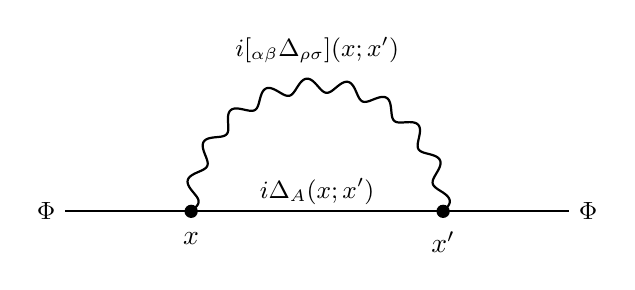
\begin{tikzpicture}[scale=1.0]
\draw[thick] (-3.2,0) -- (3.2,0);
\draw[thick, domain=0:180, samples=500, smooth, variable=\t]
  plot ({(1.6+0.09*sin(20*\t))*cos(\t)}, {(1.6+0.09*sin(20*\t))*sin(\t)});
\fill (-1.6,0) circle (2.4pt) node[below=4pt] {$x$};
\fill (1.6,0) circle (2.4pt) node[below=4pt] {$x'$};
\node[right] at (3.2,0) {\small $\Phi$};
\node[left] at (-3.2,0) {\small $\Phi$};
\node at (0,0.25) {\small $i\Delta_A(x;x')$};
\node at (0,2.05) {\small $i[{}_{\alpha\beta}\Delta_{\rho\sigma}](x;x')$};
\end{tikzpicture}
\caption{Topology of the 3-point contribution (our drawing of the content of Fig.~2 of \PI): the scalar line passes through the
two 3-point vertices at $x$ and $x'$, the graviton propagator connects them. The outer legs carry the background field $\Phi$.}
\label{fig:ch3-diagram}
\end{figure}

\paragraph{Inputs.}
\begin{itemize}[leftmargin=30pt,labelsep=5pt]
\item[(G1)] Derived Table~I and normalization \tD{} (Task~2, Chapter~1):
\begin{equation}
\begin{gathered}
\kappa\mathcal L^{(1)}=\frac12\cdot\frac1i\sum_{I=1}^2\Big[V_I^{\alpha\beta}\phi_1\phi_2\Big]_{\phi_1=\phi_2=\phi}h_{\alpha\beta},\\
V_1^{\alpha\beta}=i\kappa a^{D-2}\partial_1^\alpha\partial_2^\beta,\qquad V_2^{\alpha\beta}=-\tfrac i2\kappa a^{D-2}\eta^{\alpha\beta}\partial_1\!\cdot\partial_2 .
\end{gathered}
\label{eq:ch3-G1}
\end{equation}
\item[(G2)] Propagators \tP\,\tA:
\begin{itemize}
\item $\langle T\phi(x)\phi(x')\rangle=i\Delta_A(x;x')$. This is the Feynman propagator of the kinetic term $-\tfrac12a^{D-2}\partial\phi\cdot\partial\phi$
and satisfies \eqI{12}--\eqI{13}.
\item $\langle T\,h_{\alpha\beta}(x)h_{\rho\sigma}(x')\rangle=i[{}_{\alpha\beta}\Delta_{\rho\sigma}](x;x')$, \PI{} \eqI{20} and \eqI{25}.
\end{itemize}
Because of bosonic time ordering both propagators are symmetric under exchange:
\begin{equation*}
i\Delta_A(x;x')=i\Delta_A(x';x),\qquad i[{}_{\alpha\beta}\Delta_{\rho\sigma}](x;x')=i[{}_{\rho\sigma}\Delta_{\alpha\beta}](x';x).
\end{equation*}
\item[(G3)] Definition of $M^2$ and the effective action \tP\,\tA{} (Task~3, Chapter~2): \PI{} \eqI{168} and
\begin{equation*}
-iM^2(x;x')=\frac{\delta^2(i\Gamma_1)}{\delta\Phi(x)\,\delta\Phi(x')},\qquad e^{i\Gamma[\Phi]}=\int[Dh][D\varphi]_{\rm 1PI}\,e^{iS[\Phi+\varphi,h]}.
\end{equation*}
\end{itemize}

\paragraph{Scope.}
The substitution of the graviton propagator, i.e.\ \eqI{47}--\eqI{49} and beyond, is not part of Task~6 (it is Task~7). $D$ is general.
The singular products of propagators at $x=x'$ are defined as distributions in dimensional regularization for general $D$;
the equalities below hold in this sense, i.e.\ when integrated against test functions.

% -----------------------------------------------------------------------------------
\subsection{Effective action for the 3-point contribution \tD}

\paragraph{Background split and the cross term.}
Write $\phi=\Phi+\varphi$, with $\Phi$ the background and $\varphi$ the quantum field. Expanding the bracket in \eqref{eq:ch3-G1} produces three
kinds of terms: $\Phi\Phi h$, $\Phi\varphi h$ and $\varphi\varphi h$. Once contracted into $h_{\alpha\beta}$, the cross term can be written using the
$1\leftrightarrow2$ symmetry of $V_I$:
\begin{equation}
\big[V_I^{\alpha\beta}(\partial_1,\partial_2)\big(\Phi_1\varphi_2+\varphi_1\Phi_2\big)\big]h_{\alpha\beta}=2\big[V_I^{\alpha\beta}(\partial_1,\partial_2)\Phi_1\varphi_2\big]h_{\alpha\beta}.
\label{eq:ch3-cross}
\end{equation}
For $V_1$ this follows from $\partial_2^\alpha\partial_1^\beta h_{\alpha\beta}=\partial_1^\alpha\partial_2^\beta h_{\alpha\beta}$; $V_2$ is manifestly symmetric. Hence
\begin{equation}
S_3^{\times}=\int d^Dz\,\frac1i\sum_I\big[V_I^{\alpha\beta}(\partial_1,\partial_2)\,\Phi_1\varphi_2\big]h_{\alpha\beta}
\qquad(\text{leg 1 = outer }\Phi,\ \text{leg 2 = inner }\varphi).
\label{eq:ch3-S3x}
\end{equation}

\paragraph{Second order.}
Take $i\Gamma\supset\tfrac12\langle(iS_{\rm int})^2\rangle_{\rm c}$. The terms that are quadratic in $\Phi$ and of order $\kappa^2$ are:
\begin{enumerate}[leftmargin=18pt]
\item $\langle(iS_3^\times)^2\rangle$, with $\varphi\varphi$ and $hh$ contracted. This is Fig.~2; it is 1PI.
\item $\Phi\Phi h$ at one vertex and $\varphi\varphi h$ at the other: the graviton line ends on a scalar loop. This diagram is 1PR and is excluded.
\item $\Phi\Phi h$ together with the $\langle h\rangle$ tadpole: 1PR, excluded.
\end{enumerate}
The 4-point contribution was treated in Task~3. With \eqref{eq:ch3-S3x} and (G2),
\begin{equation*}
i\Gamma_{\rm 3pt}[\Phi]=\tfrac12\,i^2\Big(\frac1i\Big)^2\sum_{I,J}\iint d^Dz\,d^Dz'\,\big[V_I^{\alpha\beta}(z)\Phi_1\varphi_2\big]\big[V_J^{\rho\sigma}(z')\Phi_1\varphi_2\big]\;
\langle\varphi(z)\varphi(z')\rangle\,\langle h_{\alpha\beta}(z)h_{\rho\sigma}(z')\rangle .
\end{equation*}
Since $i^2(1/i)^2=1$,
\begin{equation}
\boxed{\;i\Gamma_{\rm 3pt}[\Phi]=\tfrac12\sum_{I,J}\iint d^Dz\,d^Dz'\;V_I^{\alpha\beta}(z)\,V_J^{\rho\sigma}(z')\;\Phi(z)\,\Phi(z')\;
i[{}_{\alpha\beta}\Delta_{\rho\sigma}](z;z')\;i\Delta_A(z;z')\;}
\label{eq:ch3-Gamma3}
\end{equation}
Here $\partial_1$ and $\partial'_1$ act on $\Phi(z)$ and $\Phi(z')$, while $\partial_2$ and $\partial'_2$ act on the first and second argument of $i\Delta_A$, respectively.

% -----------------------------------------------------------------------------------
\subsection{Derivation of Eq. (I.45) \tD}

\paragraph{Functional derivative and normalization.}
By (G3), $-iM^2_{\rm 3pt}(x;x')=\delta^2(i\Gamma_{\rm 3pt})/\delta\Phi(x)\delta\Phi(x')$. There are two assignments,
$(z\to x,\ z'\to x')$ and $(z\to x',\ z'\to x)$. Because of the exchange symmetry in (G2), the integrand of \eqref{eq:ch3-Gamma3} is symmetric
under $(z,I,\alpha\beta)\leftrightarrow(z',J,\rho\sigma)$, so the two assignments contribute equally. Table~\ref{tab:ch3-norm} collects all factors.

\begin{table}[h]
\centering
\begin{tabular}{lcl}
\toprule
Factor & Value & Origin\\
\midrule
cumulant expansion & $\tfrac12$ & $\tfrac12\langle(iS)^2\rangle$\\
cross term (each vertex) & $2\times2$ & Eq.~\eqref{eq:ch3-cross}\\
normalization & $(1/2i)^2$ & (G1)\\
vertex rule & $i^2$ & $e^{iS}$\\
assignments in $\delta^2$ & $2$ & $z\leftrightarrow z'$ symmetry\\
\midrule
\textbf{total} & $\mathbf{1}$ & $\tfrac12\cdot4\cdot(-\tfrac14)\cdot(-1)\cdot2=1$\\
\bottomrule
\end{tabular}
\caption{Normalization of the 3-point contribution (Task 6).}
\label{tab:ch3-norm}
\end{table}

\paragraph{Derivative rules.}
At vertex $z$, for an outer-leg derivative $\partial_{1\mu}\Phi(z)$ the functional derivative $\delta/\delta\Phi(x)$ produces $\partial^z_\mu\delta^D(z-x)$.
A partial integration in $z$ gives
\begin{equation}
\int d^Dz\;\partial^z_\mu\delta^D(z-x)\;\mathcal G(z,\ldots)=-\partial^x_\mu\,\mathcal G(x,\ldots),
\label{eq:ch3-ibp}
\end{equation}
where $\mathcal G$ is everything else that depends on $z$: $a^{D-2}(z)$, $i[\Delta](z;z')$ and $\partial_2i\Delta_A(z;z')$. The same holds at vertex $z'$.
Four rules follow:
\begin{itemize}[leftmargin=14pt]
\item \textbf{(R1)} $\partial_1\to-\partial$, acting on \emph{everything} at vertex $x$. \textbf{(R1$'$)} $\partial'_1\to-\partial'$, acting on everything at vertex $x'$.
\item \textbf{(R2)} $\partial_2\to+\partial$, acting only on $i\Delta_A(x;x')$. \textbf{(R2$'$)} $\partial'_2\to+\partial'$, acting only on $i\Delta_A$.
\end{itemize}
The product of the two outer signs is $(-1)(-1)=+1$. Therefore
{\chIIIhtag{I45}%
\begin{equation}
\boxed{\;-iM^2_{\rm 3pt}(x;x')=\sum_{I=1}^2V_I^{\alpha\beta}(x)\sum_{J=1}^2V_J^{\rho\sigma}(x')\;i[{}_{\alpha\beta}\Delta_{\rho\sigma}](x;x')\;i\Delta_A(x;x')\;}
\tag{I.45}\label{eq:ch3-45}
\end{equation}
}
with the derivatives read according to (R1)--(R2$'$) (definition sign). This is identical with \PI's \eqI{45} and with the rule stated in its text,
``partially integrate any derivative that acts upon an outer leg'' \chIIIok.

% -----------------------------------------------------------------------------------
\subsection{Comparison with the 4-point rule: the relative sign}
\label{sec:ch3-relsign}

\begin{table}[h]
\centering\small
\begin{tabular}{p{0.2\textwidth}p{0.34\textwidth}p{0.36\textwidth}}
\toprule
 & 3-point (this task) & 4-point (Task 3)\\
\midrule
position of outer legs & different vertices: $x$ and $x'$ & same vertex $x$, with $\delta^D(x-x')$\\
leg 1 & partial integration: $-\partial$, on everything & partial integration: $-\partial$, on everything\\
leg 2 & partial integration: $-\partial'$, on everything & $+\partial$ on $\delta^D(x-x')$ with respect to $x$ $(=-\partial')$\\
sign product & $(-)(-)=+$ & $(-)(+)=-$\\
paper's rule & $(-)(-)$ \chIIIok & \eqI{32}: $\partial_2\to+\partial'$, i.e.\ $(-)(-)$ \chIIIno\\
\bottomrule
\end{tabular}
\caption{Derivative rules for the outer legs in the 3-point and 4-point contributions (Task 6).}
\label{tab:ch3-rules}
\end{table}

In the 4-point contribution, once the first $\delta^D(z-x)$ has been integrated no $z$ is left for a second partial integration.
The remaining derivative acts on $\delta^D(x-x')$ with respect to the vertex coordinate $x$. In \eqI{32} the paper treats this case with
the same sign as the 3-point rule. At the end of Task~6 this was read as confirming the preliminary note of Task~3: in the paper's total result,
the 4-point contribution enters with the opposite sign relative to the 3-point contribution. (As explained in the note at the beginning of
this section, Task~9 later showed that the paper's 3-point contribution is reversed as well, from \eqI{47} on, so that the relative sign in the
paper is in fact consistent.)

% -----------------------------------------------------------------------------------
\subsection{Derivation of Eq. (I.46) \tD}

The four $(I,J)$ terms of \eqref{eq:ch3-45} are expanded with \eqref{eq:ch3-G1}. In $V_1$ it does not matter which index goes to the outer leg,
because $i[{}_{\alpha\beta}\Delta_{\rho\sigma}]$ is symmetric within the pair $\alpha\beta$. The factor $(aa')^{D-2}=a^{D-2}(x)\,a^{D-2}(x')$ belongs to the
``everything'' on which the outer derivatives act. Indices are moved with $\eta$; for example $\partial^\alpha X_{\alpha\ldots}=\partial_\alpha X^\alpha{}_{\ldots}$.
In $V_2$ we write $\partial_1\!\cdot\partial_2=\partial_1^\mu\partial_{2\mu}$ and apply (R1), $\partial_1^\mu\to-\partial^\mu$, and (R2), $\partial_{2\mu}\to\partial_\mu$.
Table~\ref{tab:ch3-IJ} shows the bookkeeping ($I$ refers to the vertex at $x$, $J$ to the vertex at $x'$).

\begin{table}[h]
\centering\small
\renewcommand{\arraystretch}{1.25}
\begin{tabular}{clllll}
\toprule
$(I,J)$ & $V$ coefficients & outer derivatives & contraction & inner & result\\
\midrule
(1,1) & $(i\kappa)(i\kappa)=-\kappa^2$ & $(-\partial^\alpha)(-\partial'^\rho)$ & $i[{}^{\alpha\beta}\Delta^{\rho\sigma}]$ & $\partial_\beta\partial'_\sigma$ & $-\kappa^2\partial_\alpha\partial'_\rho\{\ldots\}$\\
(2,1) & $(-\tfrac i2\kappa)(i\kappa)=+\tfrac{\kappa^2}2$ & $(-\partial^\mu)(-\partial'^\rho)$ & $\eta^{\alpha\beta}\to i[{}^\alpha_\alpha\Delta^{\rho\sigma}]$ & $\partial_\mu\partial'_\sigma$ & $+\tfrac{\kappa^2}2\partial^\mu\partial'_\rho\{\ldots\}$\\
(1,2) & $(i\kappa)(-\tfrac i2\kappa)=+\tfrac{\kappa^2}2$ & $(-\partial^\alpha)(-\partial'^\nu)$ & $\eta^{\rho\sigma}\to i[{}^{\alpha\beta}\Delta^\rho{}_\rho]$ & $\partial_\beta\partial'_\nu$ & $+\tfrac{\kappa^2}2\partial_\alpha\partial'^\nu\{\ldots\}$\\
(2,2) & $(-\tfrac i2\kappa)^2=-\tfrac{\kappa^2}4$ & $(-\partial^\mu)(-\partial'^\nu)$ & $i[{}^\alpha_\alpha\Delta^\rho{}_\rho]$ & $\partial_\mu\partial'_\nu$ & $-\tfrac{\kappa^2}4\partial^\mu\partial'^\nu\{\ldots\}$\\
\bottomrule
\end{tabular}
\caption{The four $(I,J)$ terms of \eqref{eq:ch3-45} (Task 6). ``Inner'' lists the derivatives that act only on $i\Delta_A$.}
\label{tab:ch3-IJ}
\end{table}

\noindent Summing the four rows:
{\chIIIhtag{I46}%
\begin{equation}
\boxed{\;
\begin{aligned}
-iM^2_{\rm 3pt}(x;x')={}&-\kappa^2\partial_\alpha\partial'_\rho\Big\{(aa')^{D-2}\,i[{}^{\alpha\beta}\Delta^{\rho\sigma}](x;x')\,\partial_\beta\partial'_\sigma i\Delta_A(x;x')\Big\}\\
&+\frac{\kappa^2}2\partial^\mu\partial'_\rho\Big\{(aa')^{D-2}\,i[{}^\alpha_\alpha\Delta^{\rho\sigma}](x;x')\,\partial_\mu\partial'_\sigma i\Delta_A(x;x')\Big\}\\
&+\frac{\kappa^2}2\partial_\alpha\partial'^\nu\Big\{(aa')^{D-2}\,i[{}^{\alpha\beta}\Delta^\rho{}_\rho](x;x')\,\partial_\beta\partial'_\nu i\Delta_A(x;x')\Big\}\\
&-\frac{\kappa^2}4\partial^\mu\partial'^\nu\Big\{(aa')^{D-2}\,i[{}^\alpha_\alpha\Delta^\rho{}_\rho](x;x')\,\partial_\mu\partial'_\nu i\Delta_A(x;x')\Big\}
\end{aligned}\;}
\tag{I.46}\label{eq:ch3-46}
\end{equation}
}
(definition sign). All coefficients are independent of $D$; $D$ appears only through $(aa')^{D-2}$ and inside the propagators.

% -----------------------------------------------------------------------------------
\subsection{Independent analytic cross-checks}

\paragraph{Textbook comparison \tA\,\tC.}
In the cubic theory $\mathcal L_{\rm int}=\tfrac g2\phi^2\chi$, the normalization used here gives the vertex $V=2i\cdot\tfrac g2=ig$. The one-loop $\phi$
self-energy is, by the standard result, $V^2\times\Delta_\phi\times\Delta_\chi$ with symmetry factor $1$. This is the same normalization as in \eqref{eq:ch3-45}.

\paragraph{Consistency with the flat-space limit (observation).}
The flat-space 3-point expression in \PI's \eqI{175}\footnote{The Task~6 report cites this expression as (174). In the printed paper
(p.~124005-15, right column) \eqI{174} is the flat-space limit of the 4-point contribution, and the flat-space 3-point expression is \eqI{175};
the reference has been corrected here.} has the same structure and the same signs as \eqI{46} ($-\kappa^2$, $+\tfrac{\kappa^2}2$, $+\tfrac{\kappa^2}2$,
$-\tfrac{\kappa^2}4$). This shows that \eqI{46} is used consistently within the paper.

% -----------------------------------------------------------------------------------
\subsection{Code checks \tC}
\label{sec:ch3-t6-code}

The script \chIIIcode{check\_45\_46.py} (SymPy and mpmath; about 3 minutes) performs three checks. It does not replace the analytic derivation above.
\begin{itemize}[leftmargin=14pt]
\item \textbf{(a) Index algebra.}
Set-up: $D=3$; a generic tensor $X_{\alpha\beta\rho\sigma}(x;x')$, symmetric within each pair, with 36 independent components
(no pair-exchange symmetry is assumed, since $x\ne x'$); derivatives represented by formal vectors ($P,P'$ outer, $Q,Q'$ inner).
With (R1)--(R2$'$), $\sum_{IJ}V_IV_JX$ is identical to \eqI{46}: \texttt{True} \chIIIok.
With $V_1\to-V_1$, i.e.\ with the printed left-hand side of \eqI{7}, the identity fails; the difference is exactly the sign reversal of the
2nd and 3rd terms (\texttt{difference = -2*(t2+t3): True}).
\item \textbf{(b) Normalization.} $\tfrac12\cdot2\cdot2\cdot(1/2i)^2\cdot i^2\cdot2=1$ \chIIIok.
\item \textbf{(c) Derivative rules with test functions.}
Set-up: a one-dimensional toy model, $i\Gamma=\tfrac12\iint W(z,z')\Phi'(z)\Phi'(z')$, with $W$ built from explicit smooth symmetric kernels,
\begin{equation*}
\begin{gathered}
W=C(z)\,C(z')\,G(z,z')\,\partial_z\partial_{z'}\Delta_\ell(z,z'),\\
C(u)=1+u^2,\qquad G=(1+zz')\,e^{-(z-z')^2/2},\qquad \Delta_\ell=e^{-(z-z')^2},
\end{gathered}
\end{equation*}
where $C$ plays the role of $a^{D-2}$, $G$ that of the graviton propagator and $\Delta_\ell$ that of the scalar propagator; the test functions are
$f_1=e^{-z^2}$ and $f_2=z\,e^{-(z-1)^2}$.
The Gateaux second derivative is $0.779492709611$; the kernel of the rule of \eqI{45}, $(-\partial_z)(-\partial_{z'})$ acting on everything, gives the
same value \chIIIok. A rule that takes one outer leg with the opposite sign (the type of rule used in \eqI{32}) gives $-0.779492709611$ \chIIIno.
\end{itemize}
Output (re-run for these notes; identical with the output recorded in Task~6):
{\footnotesize
\begin{verbatim}
== (a) index algebra (45) -> (46), D=3, generic within-pair-symmetric X_{ab rs}(x;x') ==
  Sum_IJ V_I(x) V_J(x') X  ==  (46)  with derived V_1 = +i kappa ...  : True
  with the sign of (7)'s printed LHS (V_1 = -i kappa ...)            : False
                                       (difference = -2*(t2+t3): True )
== (b) normalization: (1/2) * 2 * 2 * (1/2i)^2 * i^2 * 2 ==
  factor = 1
== (c) derivative rules, 1D toy with explicit smooth kernels and test functions ==
  Gateaux  d^2(i Gamma)/de1 de2 = 0.779492709611
  (45) rule  int f1 K f2        = 0.779492709611   equal: True
  one outer leg with + sign     = -0.779492709611   equal: False
\end{verbatim}
}
\noindent(The third line of (a) is wrapped here; the script prints it as one line.)

% -----------------------------------------------------------------------------------
\subsection{Comparison with the paper}
\label{sec:ch3-t6-compare}

\begin{table}[h]
\centering\small
\renewcommand{\arraystretch}{1.2}
\begin{tabular}{p{0.3\textwidth}p{0.42\textwidth}p{0.12\textwidth}c}
\toprule
Item & Derived & Paper & \\
\midrule
\eqI{45}: normalization & $1$ (Table~\ref{tab:ch3-norm}) & $1$ & \chIIIok\\
\eqI{45}: structure $V(x)V(x')\,i[\Delta](x;x')$ $\times\,i\Delta_A(x;x')$ & Eq.~\eqref{eq:ch3-45} & same & \chIIIok\\
outer-leg rule & $-\partial$ (on everything), at both vertices & ``partially integrate'' & \chIIIok\\
inner-leg rule & $+\partial$, only on $i\Delta_A$ & same & \chIIIok\\
\eqI{46}, 1st term & $-\kappa^2\partial_\alpha\partial'_\rho\{\ldots i[{}^{\alpha\beta}\Delta^{\rho\sigma}]\ldots\}$ & same & \chIIIok\\
\eqI{46}, 2nd term & $+\tfrac{\kappa^2}2\partial^\mu\partial'_\rho\{\ldots i[{}^\alpha_\alpha\Delta^{\rho\sigma}]\ldots\}$ & same & \chIIIok\\
\eqI{46}, 3rd term & $+\tfrac{\kappa^2}2\partial_\alpha\partial'^\nu\{\ldots i[{}^{\alpha\beta}\Delta^\rho{}_\rho]\ldots\}$ & same & \chIIIok\\
\eqI{46}, 4th term & $-\tfrac{\kappa^2}4\partial^\mu\partial'^\nu\{\ldots i[{}^\alpha_\alpha\Delta^\rho{}_\rho]\ldots\}$ & same & \chIIIok\\
\bottomrule
\end{tabular}
\caption{Task 6: comparison with \PI.}
\label{tab:ch3-t6-comp}
\end{table}

\begin{resultbox}[Conclusion (Task 6)]
\eqI{45} and \eqI{46} agree exactly with the derivation; there is no discrepancy.
The printed \eqI{46} is consistent with the derived $V_1=+i\kappa\ldots$. This agrees with the finding of Task~2: the $-\tfrac12\kappa$ on the
left-hand side of \eqI{7} is only a typographical error.
\end{resultbox}

\paragraph{Consequence of the relative sign (as assessed in Task 6).}
The paper's 3-point rule agrees with the definitions; its 4-point rule \eqI{32} does not (Sec.~\ref{sec:ch3-relsign}). Accordingly, in the paper's sum
$-iM^2=-iM^2_{\rm 4pt}+(-iM^2_{\rm 3pt})+(\text{counterterms})$, \eqI{44} appears with the opposite of its correct sign.
Task~6 proposed to determine the effect on the renormalized result as follows: multiply the paper's \eqI{44} by $-1$ (and drop the $\mp2$ terms that
originate from \eqI{40}), then redo the 3-point contributions and the counterterm adjustment of Part~IV. According to Task~5, the terms
$3\ln(aa')a^D\square$, $-4\ln(aa')a^{D-2}\nabla^2$ and $9H^2a^D$ are not of counterterm form; the sign could therefore affect the final finite result.
(This plan was overtaken by Tasks~7 and~9; see the note at the start of this section.)

\paragraph{Accumulated findings (Tasks 2--6).}
Identifiers in parentheses (S$n$, B$n$, C$n$) refer to the classified list of findings in Chapter~\ref{ch:summary}.
\begin{center}\small
\renewcommand{\arraystretch}{1.2}
\begin{tabular}{p{0.16\textwidth}p{0.4\textwidth}p{0.36\textwidth}}
\toprule
Location & Finding & Effect\\
\midrule
\eqI{7}, left side (C3) & $-\tfrac12\kappa$ printed, correct is $+\tfrac12\kappa$ & none; \eqI{46} was built with the correct $V_1$\\
Table II, $U_2$ (C5) & $-\tfrac i4$ printed, correct is $+\tfrac i4$ & none; \eqI{33} was built with the correct value\\
\eqI{32}--\eqI{33} (S1) & overall sign reversed because of the $\partial_2$ rule & at the time: \emph{confirmed} that the 4-point contribution enters with the opposite sign relative to the 3-point one (later revised, see above)\\
\eqI{39} (C6) & $\bar\eta_{\rho\sigma}\to\bar\eta^{\rho\sigma}$ & none\\
\eqI{40} (B1) & finite part $+2$ printed, correct is $-2$ & carried into \eqI{41} and \eqI{44}; absorbable into counterterms\\
\eqI{41}$\to$\eqI{44} & algebra of \eqI{42}--\eqI{43} correct & ---\\
\eqI{45}--\eqI{46} & exact agreement & ---\\
\bottomrule
\end{tabular}
\end{center}

% -----------------------------------------------------------------------------------
\subsection{Calculation record (Task 6)}
\begin{itemize}[leftmargin=14pt]
\item \textbf{Derived.} Background split and cross term, Eqs.~\eqref{eq:ch3-cross}--\eqref{eq:ch3-S3x}.
The 3-point effective action \eqref{eq:ch3-Gamma3}; the reason for excluding the 1PR contributions.
Normalization table (Table~\ref{tab:ch3-norm}). Outer- and inner-leg derivative rules \eqref{eq:ch3-ibp} and (R1)--(R2$'$).
\eqI{45} [Eq.~\eqref{eq:ch3-45}]. The origin of the sign difference between the 3- and 4-point rules (Sec.~\ref{sec:ch3-relsign}).
\eqI{46} [Eq.~\eqref{eq:ch3-46}]: the four $(I,J)$ terms with explicit coefficients and contractions.
\item \textbf{Checks passed.} Textbook normalization; SymPy/mpmath (a) index algebra, (b) normalization, (c) derivative rule with test
functions (\chIIIcode{check\_45\_46.py}). All were actually run.
\item \textbf{Discrepancies.} None in \eqI{45} and \eqI{46}.
\item \textbf{Point established in Task 6.} In \PI{} the 4-point and 3-point contributions are built with different derivative rules; the 4-point
contribution is reversed (with respect to the definitions). \emph{Later revision:} Task~9 showed that the 3-point contribution is reversed as well,
through \eqI{47}--\eqI{49}, so the relative sign is consistent.
\item \textbf{Open point (at the time).} The effect on the renormalized result; to be checked in the continuation of the 3-point computation and in Part~IV.
\end{itemize}

% ===================================================================================
\section{Task 7: inserting the graviton propagator, Eqs. (I.47)--(I.49)}
\label{sec:ch3-task7}
% ===================================================================================

\begin{discbox}[Summary of findings (Task 7)]
\begin{itemize}[leftmargin=12pt]
\item All nine terms of \eqI{47}--\eqI{49} were derived. Their structures, the $D$-dependent coefficients $\tfrac{D-1}{D-3}$ and $\tfrac{2(D-2)}{D-3}$,
and the magnitudes agree with the paper.
\item \textbf{The overall sign is reversed in all nine terms:} the derived \eqI{47}--\eqI{49} are exactly $-1$ times the printed ones.
The result was obtained along two independent routes: from the paper's \eqI{46}, and directly from \eqI{45} with Table~I.
Hence the printed \eqI{47}--\eqI{49} are inconsistent with the paper's own \eqI{46}.
\item In the $AA$ sector an extra pair of the form $\partial_i\partial'_j\{\ldots(\partial_i\partial'_j-\partial_j\partial'_i)i\Delta_A\}$ appears at an intermediate step.
It vanishes identically because of the spatial homogeneity of $i\Delta_A$ ($\partial'_ii\Delta_A=-\partial_ii\Delta_A$). The paper does not write it either.
\item \textbf{Significance.} If the signs of \eqI{47}--\eqI{49} were used in the subsequent steps, the paper's 3-point contribution is, like the
4-point contribution, reversed overall. The relative sign of the two contributions is then consistent, but the overall sign of the bare $M^2$ is
opposite to the convention of \eqI{168} and \eqI{131}. This was to be checked with Table~III and beyond (it was, in Task~9: see Sec.~\ref{sec:ch3-t7-assess}).
\end{itemize}
\end{discbox}

% -----------------------------------------------------------------------------------
\subsection{Goal, inputs, scope and notation}

\paragraph{Targets \tP.}
\PI, p.~124005-5 (introductory sentence in the left column, equations in the right column; all symbols legible), prints, with the paper's square brackets:
\begin{align}
&\kappa^2\nabla\!\cdot\!\nabla'\big[(aa')^{D-2}i\Delta_A\nabla\!\cdot\!\nabla'i\Delta_A\big]-\kappa^2\Big(\frac{D-1}{D-3}\Big)\partial_0\partial'_0\big[(aa')^{D-2}i\Delta_A\partial_0\partial'_0i\Delta_A\big]\notag\\
&\quad+\kappa^2\partial_i\partial'_0\big[(aa')^{D-2}i\Delta_A\partial_i\partial'_0i\Delta_A\big]+\kappa^2\partial_0\partial'_i\big[(aa')^{D-2}i\Delta_A\partial_0\partial'_ii\Delta_A\big],
\tag*{\eqI{47}}\\[3pt]
&-\kappa^2\partial_0\partial'_0\big[(aa')^{D-2}i\Delta_B\nabla\!\cdot\!\nabla'i\Delta_A\big]-\kappa^2\partial_i\partial'_0\big[(aa')^{D-2}i\Delta_B\partial_0\partial'_ii\Delta_A\big]\notag\\
&\quad-\kappa^2\partial_0\partial'_i\big[(aa')^{D-2}i\Delta_B\partial_i\partial'_0i\Delta_A\big]-\kappa^2\nabla\!\cdot\!\nabla'\big[(aa')^{D-2}i\Delta_B\partial_0\partial'_0i\Delta_A\big],
\tag*{\eqI{48}}\\[3pt]
&2\kappa^2\Big(\frac{D-2}{D-3}\Big)\partial_0\partial'_0\big[(aa')^{D-2}i\Delta_C\partial_0\partial'_0i\Delta_A\big].
\tag*{\eqI{49}}
\end{align}
These expressions were not used as input in the derivation; they enter only in the comparison of Sec.~\ref{sec:ch3-t7-compare}.

\paragraph{Inputs.}
\begin{itemize}[leftmargin=30pt,labelsep=5pt]
\item[(G1)] The derived \eqI{46} \tD{} (Task~6, Eq.~\eqref{eq:ch3-46}). Outer derivatives ($\partial,\partial'$) act on everything, inner derivatives only on $i\Delta_A$:
\begin{equation}
\begin{aligned}
-iM^2_{\rm 3pt}={}&-\kappa^2\partial_\alpha\partial'_\rho\{(aa')^{D-2}X^{\alpha\beta\rho\sigma}\partial_\beta\partial'_\sigma i\Delta_A\}
+\tfrac{\kappa^2}2\partial^\mu\partial'_\rho\{(aa')^{D-2}X^\alpha{}_\alpha{}^{\rho\sigma}\partial_\mu\partial'_\sigma i\Delta_A\}\\
&+\tfrac{\kappa^2}2\partial_\alpha\partial'^\nu\{(aa')^{D-2}X^{\alpha\beta\rho}{}_\rho\partial_\beta\partial'_\nu i\Delta_A\}
-\tfrac{\kappa^2}4\partial^\mu\partial'^\nu\{(aa')^{D-2}X^\alpha{}_\alpha{}^\rho{}_\rho\partial_\mu\partial'_\nu i\Delta_A\},
\end{aligned}
\label{eq:ch3-t7G1}
\end{equation}
with $X^{\alpha\beta\rho\sigma}\equiv i[{}^{\alpha\beta}\Delta^{\rho\sigma}](x;x')$.
\item[(G2)] The graviton propagator \tP, \eqI{20}--\eqI{24}: $X_{\alpha\beta\rho\sigma}=\sum_{I=A,B,C}T^I_{\alpha\beta\rho\sigma}\,i\Delta_I(x;x')$ with
\begin{equation}
\begin{aligned}
&T^A_{\alpha\beta\rho\sigma}=2\bar\eta_{\alpha(\rho}\bar\eta_{\sigma)\beta}-\tfrac{2}{D-3}\bar\eta_{\alpha\beta}\bar\eta_{\rho\sigma},\qquad
T^B_{\alpha\beta\rho\sigma}=-4\delta^0_{(\alpha}\bar\eta_{\beta)(\rho}\delta^0_{\sigma)},\\
&T^C_{\alpha\beta\rho\sigma}=\tfrac{2}{(D-2)(D-3)}\big[(D-3)\delta^0_\alpha\delta^0_\beta+\bar\eta_{\alpha\beta}\big]\big[(D-3)\delta^0_\rho\delta^0_\sigma+\bar\eta_{\rho\sigma}\big].
\end{aligned}
\label{eq:ch3-T}
\end{equation}
The $T^I$ are constant tensors; therefore $i\Delta_I(x;x')$ stays inside the bracket on which the outer derivatives act.
\item[(G3)] Tensor tools \tD{} (Task~4, Chapter~2): $u_\mu=\delta^0_\mu$, $u^\mu=-\delta^\mu_0$, $\bar\eta_{\mu\nu}=\eta_{\mu\nu}+u_\mu u_\nu$.
For vectors $V,W$: $u\cdot V=-V_0$ and $\bar\eta_{\mu\nu}V^\mu W^\nu=\bar V\!\cdot\!\bar W\equiv\sum_iV_iW_i$. Traces:
\begin{equation}
\begin{aligned}
&\eta^{\alpha\beta}T^A_{\alpha\beta\mu\nu}=-\tfrac{4}{D-3}\bar\eta_{\mu\nu},\qquad \eta^{\alpha\beta}T^B_{\alpha\beta\mu\nu}=0,\qquad \eta^{\alpha\beta}T^C_{\alpha\beta\mu\nu}=\tfrac{4}{(D-2)(D-3)}f_{\mu\nu},\\
&\eta^{\alpha\beta}\eta^{\rho\sigma}T^{A,B,C}_{\alpha\beta\rho\sigma}=-\tfrac{4(D-1)}{D-3},\ \ 0,\ \ \tfrac{8}{(D-2)(D-3)},
\end{aligned}
\label{eq:ch3-traces}
\end{equation}
where $f_{\mu\nu}\equiv(D-3)u_\mu u_\nu+\bar\eta_{\mu\nu}$.
\item[(G4)] Homogeneity of $i\Delta_A$ \tP\,\tD: by \eqI{11} and \eqI{13}, $i\Delta_A=A(y)+k\ln(aa')$, which depends on $\vec x,\vec x'$ only through $\|\vec x-\vec x'\|$. Hence
\begin{equation}
\partial'_i\,i\Delta_A=-\partial_i\,i\Delta_A,\qquad \partial_i\partial'_j\,i\Delta_A=\partial_j\partial'_i\,i\Delta_A .
\label{eq:ch3-hom}
\end{equation}
\end{itemize}

\paragraph{Scope and notation.}
Eq.~\eqI{50} and beyond (the $y$ representation and the local/logarithm/normal split) are not part of Task~7. $D$ is general; at no step is $D=4$ set.
As a shorthand we write
\begin{equation}
\chIIIbr{\partial_a\partial'_c}{\partial_b\partial'_d}{I}\equiv\partial_a\partial'_c\Big\{(aa')^{D-2}\,i\Delta_I(x;x')\,\partial_b\partial'_d\,i\Delta_A(x;x')\Big\}.
\label{eq:ch3-bracket}
\end{equation}
The derivatives on the left of the bar are outer, those on the right inner. During the computation the outer derivatives are represented by $P,P'$ and the
inner ones by $Q,Q'$; for example $P_0P'_0(\bar Q\!\cdot\!\bar Q')\to\chIIIbr{\partial_0\partial'_0}{\nabla\!\cdot\!\nabla'}{}$.

% -----------------------------------------------------------------------------------
\subsection{Term-by-term contractions \tD}

(G2) is inserted into the four terms of \eqref{eq:ch3-t7G1}. We use $T_I^{\alpha\beta\rho\sigma}P_\alpha Q_\beta P'_\rho Q'_\sigma=T^I_{\alpha\beta\rho\sigma}P^\alpha Q^\beta P'^\rho Q'^\sigma$ and (G3);
$P\!\cdot\!Q=-P_0Q_0+\bar P\!\cdot\!\bar Q$ is the Lorentz product.

\paragraph{First term: $-\kappa^2\,T^{\alpha\beta\rho\sigma}P_\alpha Q_\beta P'_\rho Q'_\sigma$.}
The contraction $T^I_{\alpha\beta\rho\sigma}P^\alpha Q^\beta P'^\rho Q'^\sigma$ (before multiplying by $-\kappa^2$) is
\begin{equation}
\begin{aligned}
T^A:&\quad (\bar P\!\cdot\!\bar P')(\bar Q\!\cdot\!\bar Q')+(\bar P\!\cdot\!\bar Q')(\bar P'\!\cdot\!\bar Q)-\tfrac{2}{D-3}(\bar P\!\cdot\!\bar Q)(\bar P'\!\cdot\!\bar Q'),\\
T^B:&\quad -\big[P_0Q'_0(\bar P'\!\cdot\!\bar Q)+Q_0Q'_0(\bar P\!\cdot\!\bar P')+P_0P'_0(\bar Q\!\cdot\!\bar Q')+Q_0P'_0(\bar P\!\cdot\!\bar Q')\big],\\
T^C:&\quad \tfrac{2}{(D-2)(D-3)}\big[(D-3)P_0Q_0+\bar P\!\cdot\!\bar Q\big]\big[(D-3)P'_0Q'_0+\bar P'\!\cdot\!\bar Q'\big].
\end{aligned}
\label{eq:ch3-c1}
\end{equation}
Used:
\begin{itemize}[leftmargin=14pt]
\item for $T^A$: $\bar\eta_{\alpha\rho}P^\alpha P'^\rho=\bar P\!\cdot\!\bar P'$ and similar;
\item for $T^B$: $(u\!\cdot\!P)(u\!\cdot\!Q')=P_0Q'_0$ and similar; the four terms come from expanding the symmetrization in \eqI{23};
\item for $T^C$: $f_{\alpha\beta}P^\alpha Q^\beta=(D-3)P_0Q_0+\bar P\!\cdot\!\bar Q$.
\end{itemize}

\paragraph{Second and third terms: one trace.}
\begin{equation}
\begin{aligned}
\tfrac{\kappa^2}2(P\!\cdot\!Q)\,\eta^{\alpha\beta}T_{\alpha\beta}{}^{\rho\sigma}P'_\rho Q'_\sigma:&\quad A:\ -\tfrac{2\kappa^2}{D-3}(P\!\cdot\!Q)(\bar P'\!\cdot\!\bar Q'),\qquad B:\ 0,\\
&\quad C:\ \tfrac{2\kappa^2}{(D-2)(D-3)}(P\!\cdot\!Q)\big[(D-3)P'_0Q'_0+\bar P'\!\cdot\!\bar Q'\big],\\[3pt]
\tfrac{\kappa^2}2(P'\!\cdot\!Q')\,T^{\alpha\beta}{}_{\rho}{}^{\rho}P_\alpha Q_\beta:&\quad A:\ -\tfrac{2\kappa^2}{D-3}(\bar P\!\cdot\!\bar Q)(P'\!\cdot\!Q'),\qquad B:\ 0,\\
&\quad C:\ \tfrac{2\kappa^2}{(D-2)(D-3)}\big[(D-3)P_0Q_0+\bar P\!\cdot\!\bar Q\big](P'\!\cdot\!Q').
\end{aligned}
\label{eq:ch3-c2}
\end{equation}
The trace in the third term has the same form as in the second because of the pair-exchange symmetry of the $T^I$ (Task~3).

\paragraph{Fourth term: double trace.}
\begin{equation}
-\tfrac{\kappa^2}4(P\!\cdot\!Q)(P'\!\cdot\!Q')\,\eta\eta T:\qquad A:\ +\kappa^2\tfrac{D-1}{D-3}(P\!\cdot\!Q)(P'\!\cdot\!Q'),\qquad B:\ 0,\qquad
C:\ -\tfrac{2\kappa^2}{(D-2)(D-3)}(P\!\cdot\!Q)(P'\!\cdot\!Q').
\label{eq:ch3-c3}
\end{equation}

% -----------------------------------------------------------------------------------
\subsection{Sorting by the type of scalar propagator \tD}

We abbreviate\footnote{The original report used the letters $a,\bar a,b,\bar b$ here; we rename them to avoid a clash with the scale factor $a$.
For the same reason its $A_{1,2},B_{1,2}$ and $c_0$ of the $AC$ sector are renamed $M_{1,2},N_{1,2}$ and $c_C$ below ($c_0$ is used in Task~8 for the first coefficient of \eqI{14}).}
$m\equiv P_0Q_0$, $\bar m\equiv\bar P\!\cdot\!\bar Q$, $n\equiv P'_0Q'_0$, $\bar n\equiv\bar P'\!\cdot\!\bar Q'$, so that $P\!\cdot\!Q=-m+\bar m$ and $P'\!\cdot\!Q'=-n+\bar n$.

\paragraph{$AA$ terms.}
Table~\ref{tab:ch3-AA} collects the $T^A$ parts of \eqref{eq:ch3-c1}--\eqref{eq:ch3-c3}.
\begin{table}[h]
\centering
\renewcommand{\arraystretch}{1.3}
\begin{tabular}{lccccc}
\toprule
Monomial & 1st term & 2nd term & 3rd term & 4th term & Total$/\kappa^2$\\
\midrule
$\bar m\,\bar n$ & $+\tfrac2{D-3}$ & $-\tfrac2{D-3}$ & $-\tfrac2{D-3}$ & $+\tfrac{D-1}{D-3}$ & $+1$\\
$m\,\bar n$ & --- & $+\tfrac2{D-3}$ & --- & $-\tfrac{D-1}{D-3}$ & $-1$\\
$\bar m\,n$ & --- & --- & $+\tfrac2{D-3}$ & $-\tfrac{D-1}{D-3}$ & $-1$\\
$m\,n$ & --- & --- & --- & $+\tfrac{D-1}{D-3}$ & $+\tfrac{D-1}{D-3}$\\
$(\bar P\!\cdot\!\bar P')(\bar Q\!\cdot\!\bar Q')$ & $-1$ & --- & --- & --- & $-1$\\
$(\bar P\!\cdot\!\bar Q')(\bar P'\!\cdot\!\bar Q)$ & $-1$ & --- & --- & --- & $-1$\\
\bottomrule
\end{tabular}
\caption{Coefficients of the $AA$ monomials (Task 7).}
\label{tab:ch3-AA}
\end{table}

In the first row $\tfrac{2-2-2+D-1}{D-3}=1$: the factor $D-3$ cancels exactly. The total is
\begin{equation}
\kappa^2\Big\{-(\bar P\!\cdot\!\bar P')(\bar Q\!\cdot\!\bar Q')+\tfrac{D-1}{D-3}\,mn-\bar m\,n-m\,\bar n\Big\}
+\kappa^2\Big\{\bar m\,\bar n-(\bar P\!\cdot\!\bar Q')(\bar P'\!\cdot\!\bar Q)\Big\}.
\label{eq:ch3-AAsum}
\end{equation}
The second curly bracket is $\chIIIbr{\partial_i\partial'_j}{\partial_i\partial'_j-\partial_j\partial'_i}{A}$. By (G4) the inner derivatives may be taken as
$\partial'_j=-\partial_j$; then $(\partial_i\partial'_j-\partial_j\partial'_i)i\Delta_A=-(\partial_i\partial_j-\partial_j\partial_i)i\Delta_A=0$. This pair vanishes identically.
With the mapping $\bar m\,n=P_iQ_iP'_0Q'_0\to\chIIIbr{\partial_i\partial'_0}{\partial_i\partial'_0}{}$ and $m\,\bar n=P_0Q_0P'_iQ'_i\to\chIIIbr{\partial_0\partial'_i}{\partial_0\partial'_i}{}$,
{\chIIIhtag{I47p}%
\begin{equation}
\boxed{\;
\begin{aligned}
AA:\quad&-\kappa^2\nabla\!\cdot\!\nabla'\big[(aa')^{D-2}i\Delta_A\nabla\!\cdot\!\nabla'i\Delta_A\big]\\
&+\kappa^2\Big(\frac{D-1}{D-3}\Big)\partial_0\partial'_0\big[(aa')^{D-2}i\Delta_A\partial_0\partial'_0i\Delta_A\big]\\
&-\kappa^2\partial_i\partial'_0\big[(aa')^{D-2}i\Delta_A\partial_i\partial'_0i\Delta_A\big]\\
&-\kappa^2\partial_0\partial'_i\big[(aa')^{D-2}i\Delta_A\partial_0\partial'_ii\Delta_A\big]
\end{aligned}\;}
\tag{I.47$'$}\label{eq:ch3-47}
\end{equation}
}

\paragraph{$AB$ terms.}
Since the traces of $T^B$ vanish, only the first term contributes: $-\kappa^2\times$\eqref{eq:ch3-c1}$_B$. The four monomials map as follows:
\begin{itemize}[leftmargin=14pt]
\item $P_0P'_0(\bar Q\!\cdot\!\bar Q')\to\chIIIbr{\partial_0\partial'_0}{\nabla\!\cdot\!\nabla'}{B}$;
\item $Q_0P'_0(\bar P\!\cdot\!\bar Q')\to\chIIIbr{\partial_i\partial'_0}{\partial_0\partial'_i}{B}$;
\item $P_0Q'_0(\bar P'\!\cdot\!\bar Q)\to\chIIIbr{\partial_0\partial'_i}{\partial_i\partial'_0}{B}$;
\item $Q_0Q'_0(\bar P\!\cdot\!\bar P')\to\chIIIbr{\nabla\!\cdot\!\nabla'}{\partial_0\partial'_0}{B}$.
\end{itemize}
{\chIIIhtag{I48p}%
\begin{equation}
\boxed{\;
\begin{aligned}
AB:\quad&+\kappa^2\partial_0\partial'_0\big[(aa')^{D-2}i\Delta_B\nabla\!\cdot\!\nabla'i\Delta_A\big]+\kappa^2\partial_i\partial'_0\big[(aa')^{D-2}i\Delta_B\partial_0\partial'_ii\Delta_A\big]\\
&+\kappa^2\partial_0\partial'_i\big[(aa')^{D-2}i\Delta_B\partial_i\partial'_0i\Delta_A\big]+\kappa^2\nabla\!\cdot\!\nabla'\big[(aa')^{D-2}i\Delta_B\partial_0\partial'_0i\Delta_A\big]
\end{aligned}\;}
\tag{I.48$'$}\label{eq:ch3-48}
\end{equation}
}

\paragraph{$AC$ terms.}
Define $M_1=(D-3)m+\bar m$, $M_2=-m+\bar m$, and similarly $N_1=(D-3)n+\bar n$, $N_2=-n+\bar n$. With $c_C\equiv\tfrac{2\kappa^2}{(D-2)(D-3)}$
the $C$ parts of \eqref{eq:ch3-c1}--\eqref{eq:ch3-c3} add up to
\begin{equation}
c_C\big[-M_1N_1+M_2N_1+M_1N_2-M_2N_2\big]=-c_C(M_1-M_2)(N_1-N_2)=-c_C\,(D-2)^2\,mn ,
\label{eq:ch3-ACfac}
\end{equation}
so that
{\chIIIhtag{I49p}%
\begin{equation}
\boxed{\;AC:\quad-2\kappa^2\Big(\frac{D-2}{D-3}\Big)\,\partial_0\partial'_0\big[(aa')^{D-2}i\Delta_C\,\partial_0\partial'_0\,i\Delta_A\big]\;}
\tag{I.49$'$}\label{eq:ch3-49}
\end{equation}
}
The total number of terms is $4+4+1=9$, in agreement with the paper's ``nine terms''. Eqs.~\eqref{eq:ch3-47}--\eqref{eq:ch3-49} are in the definition sign.

% -----------------------------------------------------------------------------------
\subsection{A hand check \tC}

The structure $\nabla\!\cdot\!\nabla'[\ldots\nabla\!\cdot\!\nabla'i\Delta_A]$, i.e.\ $(\bar P\!\cdot\!\bar P')(\bar Q\!\cdot\!\bar Q')$ with $i\Delta_A$ in the outer bracket,
can come from only one place: the first term of \eqref{eq:ch3-t7G1} together with the first part $\bar\eta^{\alpha\rho}\bar\eta^{\sigma\beta}$ of $T^A$. In the
other terms the outer derivative is always contracted with the inner derivative at the same point. The coefficient of the first term of
\eqref{eq:ch3-t7G1} is $-\kappa^2$, and the coefficient of the $\bar\eta\bar\eta$ part of \eqI{22} is $+1$. The coefficient is therefore unambiguously $-\kappa^2$;
the paper writes $+\kappa^2$. The other eight terms show the same overall sign difference.

% -----------------------------------------------------------------------------------
\subsection{Code checks \tC}
\label{sec:ch3-t7-code}

The script \chIIIcode{check\_47\_49.py} (about 1.5~s) builds $T^A$, $T^B$, $T^C$ as explicit component arrays for $D=4,5,6$. Outer and inner derivatives
are formal vectors ($P,Q,P',Q'$), and the scalar propagator type in the outer bracket is tracked by the symbols $d_A,d_B,d_C$. Results:
\begin{itemize}[leftmargin=14pt]
\item \textbf{(46) route $=$ (45) route}, i.e.\ directly from Table~I and \eqI{45}: \texttt{True}. This is a check that is independent of (G1).
\item (46) route $=$ derived \eqref{eq:ch3-47}--\eqref{eq:ch3-49} $+$ antisymmetric pair: \texttt{True}.
\item The antisymmetric pair vanishes with $\partial'_i=-\partial_i$ (inner derivatives): \texttt{True}.
\item (46) route $=$ printed \eqI{47}--\eqI{49}: \texttt{False}. (46) route $=-$(printed \eqI{47}--\eqI{49}): \texttt{True}.
\item Homogeneity (G4) verified explicitly with $F=A(y)+k\ln(aa')$: $\partial'_iF=-\partial_iF$, and $\partial_i\partial'_jF$ is symmetric.
\end{itemize}
Output (re-run for these notes; identical with the output recorded in Task~7; the blocks for $D=5$ and $D=6$ are identical to that for $D=4$):
{\footnotesize
\begin{verbatim}
D=4: (46)-route == (45)-route                         : True
       (46)-route == derived (47)-(49) + antisym. pair      : True
       antisym. pair vanishes when d'_i = -d_i on iDelta_A  : True
       (46)-route == paper's (47)-(49)  (after d'_i=-d_i)   : False
       (46)-route == -(paper's (47)-(49)) (after d'_i=-d_i) : True
   [D=5 and D=6: same five lines]
== homogeneity of iDelta_A: d'_i F = -d_i F and d_i d'_j F symmetric, F = A(y) + k ln(a a') ==
  d'_i F + d_i F = 0           : True
  d_i d'_j F - d_j d'_i F = 0  : True
\end{verbatim}
}

% -----------------------------------------------------------------------------------
\subsection{Comparison with the paper}
\label{sec:ch3-t7-compare}

\begin{table}[h]
\centering\small
\renewcommand{\arraystretch}{1.25}
\begin{tabular}{llll}
\toprule
Term & Derived & Paper & \\
\midrule
$AA$: $\chIIIbr{\nabla\!\cdot\!\nabla'}{\nabla\!\cdot\!\nabla'}{A}$ & $-\kappa^2$ & $+\kappa^2$ & \chIIIno{} sign\\
$AA$: $\chIIIbr{\partial_0\partial'_0}{\partial_0\partial'_0}{A}$ & $+\kappa^2\frac{D-1}{D-3}$ & $-\kappa^2\frac{D-1}{D-3}$ & \chIIIno{} sign\\
$AA$: $\chIIIbr{\partial_i\partial'_0}{\partial_i\partial'_0}{A}$ & $-\kappa^2$ & $+\kappa^2$ & \chIIIno{} sign\\
$AA$: $\chIIIbr{\partial_0\partial'_i}{\partial_0\partial'_i}{A}$ & $-\kappa^2$ & $+\kappa^2$ & \chIIIno{} sign\\
$AB$: four terms & all $+\kappa^2$ & all $-\kappa^2$ & \chIIIno{} sign\\
$AC$: $\chIIIbr{\partial_0\partial'_0}{\partial_0\partial'_0}{C}$ & $-2\kappa^2\frac{D-2}{D-3}$ & $+2\kappa^2\frac{D-2}{D-3}$ & \chIIIno{} sign\\
structures, $D$ dependence, magnitudes, 9 terms & same & same & \chIIIok\\
antisymmetric $AA$ pair & $=0$ by (G4) & not written & \chIIIok\\
\bottomrule
\end{tabular}
\caption{Task 7: comparison with \PI{} (derived terms in the definition sign).}
\label{tab:ch3-t7-comp}
\end{table}

\begin{discbox}[Conclusion (Task 7)]
Derived \eqI{47}--\eqI{49} $=-$(printed \eqI{47}--\eqI{49}), in all nine terms.
The difference cannot come from the propagator tensors: the same $T^I$ reproduced the paper's \eqI{37}--\eqI{38} exactly in Task~4. Nor can it come from the
vertices: \eqI{46} agrees with the paper. It is an overall sign inconsistency arising in the paper's step from \eqI{46} to \eqI{47}--\eqI{49}.
\end{discbox}

\subsection{Joint assessment with Tasks 3 and 6}
\label{sec:ch3-t7-assess}

At the end of Task~7 there were two possibilities:
\begin{enumerate}[leftmargin=18pt]
\item \textbf{The signs of \eqI{47}--\eqI{49} were used in the subsequent steps.} Then the paper's 3-point contribution, like the 4-point contribution,
is reversed overall with respect to the definitions. In this case the relative sign of the two contributions is consistent (both reversed), but the overall sign of
the bare $M^2$ is opposite to the convention of \eqI{168} and \eqI{131}. Since the counterterm coefficients are chosen to cancel the divergences, the renormalized
result would be $-1$ times the correct one, up to arbitrary finite local terms. This affects the sign of the mode-function correction in [30] of \PI.
(Chapter~\ref{ch:sk} later shows that at late times the non-falling total vanishes, so only decaying terms change sign and the late-time conclusion
of \PII{} is unchanged.)
\item \textbf{The sign of \eqI{46} was used in the subsequent steps.} Then the sign in \eqI{47}--\eqI{49} is only a typographical error, and the relative-sign
problem established in Tasks~3 and~6 (4-point reversed relative to 3-point) remains.
\end{enumerate}
Which one holds can be decided from the signs of the coefficients in \eqI{50}--\eqI{53} and in Tables~III--IV; this was left to the following tasks.

\begin{notebox}[Resolution (Task 9, Chapter 4)]
Task~9 found that the derived \eqI{54}, \eqI{57} and \eqI{58} are exactly $-1$ times the printed ones, while the paper's right-hand sides correctly evaluate left-hand
sides that carry the signs of the \emph{printed} \eqI{47}--\eqI{49}. Possibility~1 therefore holds: the sign error of the step \eqI{46}$\to$\eqI{47}--\eqI{49} was carried
into the subsequent computation. (Task~8, below, could not decide the question, because \eqI{50}--\eqI{53} carry no overall coefficients.)
\end{notebox}

\paragraph{Accumulated findings (Tasks 2--7).}
\begin{center}\small
\renewcommand{\arraystretch}{1.2}
\begin{tabular}{p{0.16\textwidth}p{0.42\textwidth}p{0.34\textwidth}}
\toprule
Location & Finding & Effect\\
\midrule
\eqI{7}, left side (C3) & $-\tfrac12\kappa$ printed, correct is $+\tfrac12\kappa$ & none\\
Table II, $U_2$ (C5) & $-\tfrac i4$ printed, correct is $+\tfrac i4$ & none\\
\eqI{32}--\eqI{33} (S1) & overall sign of the 4-point contribution reversed because of the $\partial_2$ rule & carried into \eqI{41} and \eqI{44}\\
\eqI{39} (C6) & $\bar\eta_{\rho\sigma}\to\bar\eta^{\rho\sigma}$ & none\\
\eqI{40} (B1) & finite part $+2$ printed, correct is $-2$ & absorbable into counterterms\\
\eqI{45}--\eqI{46} & exact agreement & ---\\
\textbf{\eqI{47}--\eqI{49}} (S1) & overall sign reversed in all nine terms (relative to the paper's \eqI{46}) & one of the two possibilities above; to be decided later (decided in Task~9: possibility~1)\\
\bottomrule
\end{tabular}
\end{center}

% -----------------------------------------------------------------------------------
\subsection{Calculation record (Task 7)}
\begin{itemize}[leftmargin=14pt]
\item \textbf{Derived.} Term-by-term contractions \eqref{eq:ch3-c1}--\eqref{eq:ch3-c3}. The $AA$ coefficient table and \eqref{eq:ch3-AAsum}. The vanishing of the
antisymmetric pair by homogeneity. \eqI{47} [Eq.~\eqref{eq:ch3-47}], \eqI{48} [Eq.~\eqref{eq:ch3-48}], \eqI{49} [Eq.~\eqref{eq:ch3-49}]; for $AC$ the factorization
$-(M_1-M_2)(N_1-N_2)$. Everything at general $D$.
\item \textbf{Checks passed.} Hand check; SymPy for $D=4,5,6$: (46) route $=$ (45) route, identity with the derived result, homogeneity
(\chIIIcode{check\_47\_49.py}). All were actually run.
\item \textbf{Discrepancy.} In \eqI{47}--\eqI{49} the overall sign is reversed in all nine terms; the paper is inconsistent with its own \eqI{46}.
\item \textbf{Open point (at the time).} Which sign was used in the subsequent steps. (Answered in Task~9: the printed sign of \eqI{47}--\eqI{49}.)
\end{itemize}

% ===================================================================================
\section{Task 8: Eqs. (I.50)--(I.53) and the derivation of (I.52)}
\label{sec:ch3-task8}
% ===================================================================================

\begin{resultbox}[Summary of findings (Task 8)]
\begin{itemize}[leftmargin=12pt]
\item \textbf{\eqI{52} verified.} The coefficient of the local term, $\delta^0_\rho\delta^0_\sigma\,\tfrac{i}{a^{D-2}}\,\delta^D(x-x')$, was obtained along three independent routes:
(A) a direct computation with the $i\delta$ prescription; (B) the propagator equation \eqI{12}; (C) the canonical equal-time commutator.
The regular part $A''(y)\,\partial_\rho y\,\partial'_\sigma y+A'(y)\,\partial_\rho\partial'_\sigma y$ follows from the chain rule. The term $k\ln(aa')$ drops out exactly under
the mixed derivatives.
\item \textbf{\eqI{50}, \eqI{51}, \eqI{53} and the three-way split (i)--(iii)} are correct. They are consistent with the nine terms derived in Task~7 and with
\eqI{13}, \eqI{27}, \eqI{28}. The split is complete and free of overlap.
\item \textbf{New typographical error: the first coefficient of \eqI{14}.} The paper prints $\Gamma(\tfrac D2-1)/(\tfrac D2-1)$; the correct value is
$\Gamma(\tfrac D2)/(\tfrac D2-1)=\Gamma(\tfrac D2-1)$. This is the value consistent with \eqI{26}, with the recursion imposed by the second coefficient of \eqI{14},
and with \eqI{52}. Had the printed value been used, the local coefficient of \eqI{52} would carry an extra factor $\tfrac{2}{D-2}$. This factor equals $1$ at
$D=4$, but multiplied by the pole of $i\Delta_A(x;x)$ it would produce a finite difference. Since the paper's \eqI{52} carries the correct coefficient, the error is
in the printing only.
\end{itemize}
\end{resultbox}

% -----------------------------------------------------------------------------------
\subsection{Goal, inputs and scope}

\paragraph{Abbreviations.}
$\Delta\eta\equiv\eta-\eta'$, $r\equiv\|\vec x-\vec x'\|$, $\mathcal N\equiv H^{D-2}/(4\pi)^{D/2}$. $\delta$ is the positive parameter of the $i\delta$ prescription in \eqI{11};
$\delta^D$ and $\delta(\Delta\eta)$ are Dirac distributions.

\paragraph{Target and comment equations \tP.}
\PI, p.~124005-5, right column, prints \eqI{50}--\eqI{53} with explanatory text (all symbols legible):
\begin{gather}
\kappa^2\partial_\mu\partial'_\nu\big[(aa')^{D-2}i\Delta_I(x;x')\partial_\rho\partial'_\sigma i\Delta_A(x;x')\big],\qquad I=A,B,C,\tag*{\eqI{50}}\\
i\Delta_A(x;x')=A(y)+k\ln(aa'),\qquad i\Delta_B(x;x')=B(y),\qquad i\Delta_C(x;x')=C(y),\tag*{\eqI{51}}\\
\partial_\rho\partial'_\sigma i\Delta_A(x;x')=\delta^0_\rho\delta^0_\sigma\,\frac{i}{a^{D-2}}\,\delta^D(x-x')+A''(y)\,\frac{\partial y}{\partial x^\rho}\frac{\partial y}{\partial x'^\sigma}
+A'(y)\,\frac{\partial^2y}{\partial x^\rho\partial x'^\sigma},\tag*{\eqI{52}}\\
\kappa^2\partial_\mu\partial'_\nu\Big\{(aa')^{D-2}I(y)\Big[A''\frac{\partial y}{\partial x^\rho}\frac{\partial y}{\partial x'^\sigma}+A'\frac{\partial^2y}{\partial x^\rho\partial x'^\sigma}\Big]\Big\}.\tag*{\eqI{53}}
\end{gather}
The text states that each of the nine terms of \eqI{47}--\eqI{49} has the form \eqI{50}; that the three propagators are almost entirely functions of $y$, \eqI{51}, with
$A$, $B$, $C$ read off from \eqI{14}, \eqI{27}, \eqI{28}; that the inner derivatives eliminate the de Sitter breaking term of $i\Delta_A$, \eqI{52}; and that the analysis
splits into (i) local contributions from the delta function in \eqI{52}, (ii) logarithm contributions from $k\ln(aa')$ in the $A$-type propagator when $I=A$ in \eqI{50},
and (iii) normal contributions \eqI{53}. The only equation that needs a derivation is \eqI{52}; it was not used as input, and enters only in the comparison of
Sec.~\ref{sec:ch3-t8-compare}.

\paragraph{Inputs.}
\begin{itemize}[leftmargin=30pt,labelsep=5pt]
\item[(G1)] \eqI{11} \tP: $y=aa'H^2\{r^2-(|\Delta\eta|-i\delta)^2\}$, $a=-1/(H\eta)$; hence $\partial_0a=Ha^2$.
\item[(G2)] \eqI{13} \tP: $i\Delta_A=A(y)+k\ln(aa')$. From \eqI{14} \emph{only} the structure
\begin{equation}
A(y)=\mathcal N\Big\{c_0\Big(\frac4y\Big)^{\frac D2-1}+c_1\Big(\frac4y\Big)^{\frac D2-2}+\ldots\Big\}
\label{eq:ch3-Astruct}
\end{equation}
is taken; the remaining terms are a constant, powers $y^n$ ($n\ge1$) and $y^{n-\frac D2+2}$ ($n\ge1$). The coefficient $c_0$ is determined separately in Sec.~\ref{sec:ch3-c0}.
The first line of \eqI{14} (p.~124005-2) prints $c_0=\Gamma(\tfrac D2-1)/(\tfrac D2-1)$ and $c_1=\Gamma(\tfrac D2+1)/(\tfrac D2-2)$.
\item[(G3)] \eqI{26} \tP: $i\Delta_{\rm cf}=\mathcal N\,\Gamma(\tfrac D2-1)(4/y)^{\frac D2-1}$. According to the text of \PI{} this is the most singular part of the scalar propagator.
\item[(G4)] \eqI{12} \tP: $\partial_\mu\big(a^{D-2}\eta^{\mu\nu}\partial_\nu\big)i\Delta_A(x;x')=i\delta^D(x-x')$. Used only in route B.
\item[(G5)] Canonical quantization \tA: from $\mathcal L=-\tfrac12a^{D-2}\eta^{\mu\nu}\partial_\mu\phi\partial_\nu\phi$ in \eqI{1},
\begin{equation*}
\pi=a^{D-2}\dot\phi,\qquad [\phi(\eta,\vec x),\pi(\eta,\vec x')]=i\delta^{D-1}(\vec x-\vec x');
\end{equation*}
moreover $i\Delta_A=\langle T\phi(x)\phi(x')\rangle$. Used only in route C.
\end{itemize}

\paragraph{Meaning of the equality \tA.}
For fixed $\delta>0$, $i\Delta_A$ is smooth in the spatial coordinates; in time it has only the kink of $|\Delta\eta|$ at $\Delta\eta=0$ (Sec.~\ref{sec:ch3-kink}).
Therefore \eqI{52} is established as an exact distributional identity at fixed $\delta>0$. The limit $\delta\to0$ is taken at the very end: the singular part tends to $\delta^D$,
and the regular part is understood through its pointwise limit. Products of the regular part with $i\Delta_I$ are defined by dimensional regularization, as the paper does from
\eqI{146} on. $D$ is general everywhere.

% -----------------------------------------------------------------------------------
\subsection{Assessment of the comment equations}

\paragraph{Eq. (I.50) \tC.}
Claim: each of the nine terms in \eqI{47}--\eqI{49} has the form
\begin{equation*}
\kappa^2\partial_\mu\partial'_\nu\big[(aa')^{D-2}i\Delta_I\,\partial_\rho\partial'_\sigma i\Delta_A\big].
\end{equation*}
Each of the nine terms derived in Task~7, Eqs.~\eqref{eq:ch3-47}--\eqref{eq:ch3-49}, contains exactly one outer $\partial$ (at $x$) and one outer $\partial'$ (at $x'$), and the
inner derivative pair is always of the form $\partial_\rho\partial'_\sigma$ (for $\nabla\!\cdot\!\nabla'$: $\mu=\nu=i$, summed over $i$). The claim is therefore correct \chIIIok.
\eqI{50} is a coefficient-free statement of form; it is not affected by the overall-sign question of Task~7.

\paragraph{Eq. (I.51) \tC.}
$i\Delta_A=A(y)+k\ln(aa')$ repeats \eqI{13}. $i\Delta_B=B(y)$ and $i\Delta_C=C(y)$ are read off directly from \eqI{27}--\eqI{28}: the right-hand sides depend on $x,x'$ only
through $y$ and contain no $\ln(aa')$. The exception in the phrase ``almost entirely functions of $y$'' is the $k\ln(aa')$ of $i\Delta_A$ \chIIIok.
Note: $A(y)$ is ``read off from \eqI{14}''; for the typographical error in the first coefficient of \eqI{14} see Sec.~\ref{sec:ch3-c0}.

\paragraph{``The inner derivatives eliminate the de Sitter breaking term'' \tD.}
\begin{equation}
\partial_\rho\partial'_\sigma\,k\ln(aa')=k\,\partial_\rho\partial'_\sigma\big[\ln a(\eta)+\ln a(\eta')\big]=0,
\label{eq:ch3-lnkill}
\end{equation}
because each summand depends on only one of the two points. The inner derivatives are always mixed ($\partial$ and $\partial'$), so the claim is correct \chIIIok.
The $\ln(aa')$ in the outer factor $i\Delta_I$ survives; this is exactly item (ii) of the split.

\paragraph{The three-way split (i)--(iii) and (I.53) \tC.}
Inserting \eqI{52} into \eqI{50} splits every term into three parts:
\begin{equation}
\begin{aligned}
&\kappa^2\partial_\mu\partial'_\nu\Big[(aa')^{D-2}i\Delta_I\Big(\underbrace{\delta^0_\rho\delta^0_\sigma\tfrac{i}{a^{D-2}}\delta^D}_{\text{(i) local}}
+\underbrace{A''\partial_\rho y\,\partial'_\sigma y+A'\partial_\rho\partial'_\sigma y}_{\equiv\mathcal R_{\rho\sigma}}\Big)\Big],\\[4pt]
&i\Delta_I\,\mathcal R=\begin{cases}\underbrace{A(y)\mathcal R}_{\text{(iii)}}+\underbrace{k\ln(aa')\mathcal R}_{\text{(ii)}},& I=A,\\[2pt] \underbrace{I(y)\mathcal R}_{\text{(iii)}},& I=B,C.\end{cases}
\end{aligned}
\label{eq:ch3-split}
\end{equation}
\begin{itemize}[leftmargin=14pt]
\item \textbf{(i) Local contributions.} Because of $\delta^D(x-x')$, $i\Delta_I(x;x')\to i\Delta_I(x;x)$. These are the coincidence limits of Task~4, including $2k\ln a$ for
$I=A$. Only the terms with the inner derivative pair $\partial_0\partial'_0$ contribute. There are three of them: the second term of $AA$, the fourth term of $AB$
($\nabla\!\cdot\!\nabla'[\ldots i\Delta_B\partial_0\partial'_0i\Delta_A]$), and the $AC$ term.\\
\emph{Later note (Task~9, Chapter~4):} \PI{} uses only $A(y)$ in the local contribution for $I=A$ and assigns the piece $k\ln(aa')\times\delta^D$ to the
logarithm contributions \eqI{60}--\eqI{67}. Both assignments are complete; Task~9 adopted the paper's for the comparison.
\item \textbf{(ii) Logarithm contributions.} For $I=A$: the product of the $k\ln(aa')$ in the outer $i\Delta_A$ with the regular part. The local part is counted in (i), so there is no double counting.
\item \textbf{(iii) Normal contributions.} $I(y)\,\mathcal R_{\rho\sigma}$, where for $I=A$ one takes $I(y)=A(y)$ (without the logarithm). This is \eqI{53} \chIIIok.
\end{itemize}
Result: the split is complete (no piece is left out) and free of overlap. \eqI{53} is nothing but the insertion of the regular part of \eqI{52} into \eqI{50}.

% -----------------------------------------------------------------------------------
\subsection{Derivation of Eq. (I.52), route A: directly with the $i\delta$ prescription \tD}

\paragraph{Structure of $y$ and analyticity of $A(y)$.}
For $\delta>0$,
\begin{equation}
y=aa'H^2\big\{r^2-\Delta\eta^2+2i\delta|\Delta\eta|+\delta^2\big\},\qquad \mathrm{Im}\,y=2aa'H^2\delta|\Delta\eta|\ge0 .
\label{eq:ch3-ystruct}
\end{equation}
$\mathrm{Im}\,y=0$ only for $\Delta\eta=0$, and then $y=aa'H^2(r^2+\delta^2)>0$. Hence $y$ neither vanishes nor reaches the negative real axis.
The powers in $A(y)$ ($y^{1-D/2}$, $y^{2-D/2}$, \ldots) are analytic on the principal branch, and for $\delta>0$ the derivatives are defined pointwise.
The only non-smooth structure is $|\Delta\eta|$.

\paragraph{Chain rule and the kink lemma.}
\label{sec:ch3-kink}
The distributional derivatives of $|\Delta\eta|$ are $\partial_0|\Delta\eta|=\mathrm{sgn}(\Delta\eta)$, $\partial'_0|\Delta\eta|=-\mathrm{sgn}(\Delta\eta)$ and
$\partial'_0\,\mathrm{sgn}(\Delta\eta)=-2\delta(\Delta\eta)$. Hence
\begin{equation}
\partial_0\partial'_0\big(|\Delta\eta|-i\delta\big)^2=\partial_0\partial'_0\big(\Delta\eta^2-2i\delta|\Delta\eta|-\delta^2\big)
=-2-2i\delta\,\partial_0\big(-\mathrm{sgn}\,\Delta\eta\big)=-2+4i\delta\,\delta(\Delta\eta).
\label{eq:ch3-kinklemma}
\end{equation}
The other components: $\partial'_jy=-2aa'H^2(x-x')_j$ contains no $|\Delta\eta|$, so $\partial_0\partial'_jy$, $\partial_i\partial'_0y$ and $\partial_i\partial'_jy$ carry no
distributional term. In the product $A''\partial_\rho y\,\partial'_\sigma y$ only $\mathrm{sgn}^2=1$ appears. Derivatives acting on the factors $a$ and $a'$ are smooth. Therefore
\begin{equation}
\partial_\rho\partial'_\sigma A(y)=A''(y)\,\partial_\rho y\,\partial'_\sigma y+A'(y)\big[\partial_\rho\partial'_\sigma y\big]_{\rm reg}
+\delta^0_\rho\delta^0_\sigma\,A'(y)\big(-aa'H^2\big)\,4i\delta\,\delta(\Delta\eta).
\label{eq:ch3-chain}
\end{equation}
In the last term $\delta(\Delta\eta)$ allows us to set $a'=a$ and $y=a^2H^2(r^2+\delta^2)$:
\begin{equation}
\mathcal S_\delta\equiv-4i\delta\,a^2H^2\,A'\big(a^2H^2(r^2+\delta^2)\big)\,\delta(\Delta\eta).
\label{eq:ch3-Sdelta}
\end{equation}

\paragraph{The limit $\delta\to0$.}
\textbf{Lemma (nascent delta function).} In $D-1$ dimensions, in the sense of distributions,
\begin{equation}
\lim_{\delta\to0^+}\ \delta\,(r^2+\delta^2)^{-D/2}=\frac{\pi^{D/2}}{\Gamma(\frac D2)}\,\delta^{D-1}(\vec x-\vec x').
\label{eq:ch3-nascent}
\end{equation}
\emph{Proof.} With the rescaling $r=\delta s$ the weight concentrates at the origin as $\delta\to0$. The total weight is
\begin{equation*}
\Omega_{D-2}\int_0^\infty s^{D-2}(1+s^2)^{-D/2}ds=\frac{2\pi^{\frac{D-1}2}}{\Gamma(\frac{D-1}2)}\cdot\frac12B\big(\tfrac{D-1}2,\tfrac12\big)=\frac{\pi^{D/2}}{\Gamma(\frac D2)} .
\end{equation*}

\noindent\textbf{Leading term.} Since $A'\supset\mathcal N c_0(1-\tfrac D2)4^{\frac D2-1}y^{-D/2}$, \eqref{eq:ch3-Sdelta} becomes
\begin{equation}
\mathcal S_\delta\supset4i\,\mathcal Nc_0\big(\tfrac D2-1\big)4^{\frac D2-1}(aH)^{2-D}\;\delta(r^2+\delta^2)^{-D/2}\,\delta(\Delta\eta)
\ \xrightarrow{\ \delta\to0\ }\ i\,\frac{c_0(\frac D2-1)}{\Gamma(\frac D2)}\,a^{2-D}\,\delta^D(x-x'),
\label{eq:ch3-lead}
\end{equation}
where $\mathcal N\,4^{\frac D2}\,H^{2-D}\,\pi^{D/2}=1$ was used. For $c_0=\Gamma(\tfrac D2-1)$ (see Sec.~\ref{sec:ch3-c0}), $c_0(\tfrac D2-1)=\Gamma(\tfrac D2)$ and the coefficient is exactly $i\,a^{2-D}$.

\noindent\textbf{Subleading terms.} The other terms of $A'$ are at most as singular as $y^{1-D/2}$. The $d^{D-1}x$ integral of $\delta\,(r^2+\delta^2)^{1-D/2}$ is $O(\delta)$;
these terms therefore vanish in the limit.

\paragraph{Result.}
Combining \eqref{eq:ch3-lnkill}, \eqref{eq:ch3-chain} and \eqref{eq:ch3-lead}:
{\chIIIhtag{I52}%
\begin{equation}
\boxed{\;\partial_\rho\partial'_\sigma i\Delta_A(x;x')=\delta^0_\rho\delta^0_\sigma\,\frac{i}{a^{D-2}}\,\delta^D(x-x')+A''(y)\,\frac{\partial y}{\partial x^\rho}\frac{\partial y}{\partial x'^\sigma}
+A'(y)\,\frac{\partial^2y}{\partial x^\rho\partial x'^\sigma}\;}
\tag{I.52}\label{eq:ch3-52}
\end{equation}
}
The $\partial^2y/\partial x^\rho\partial x'^\sigma$ in the last term is the regular part in \eqref{eq:ch3-chain}; as $\delta\to0$ it is, pointwise, the derivative of the $\delta=0$ form of \eqI{11}.
This is identical with the paper's \eqI{52} \chIIIok.

% -----------------------------------------------------------------------------------
\subsection{Independent derivations of the local coefficient}

\paragraph{Route B: from the propagator equation (independent of the normalization) \tD.}
Let $G(x;x')$ depend on time through $|\Delta\eta|$ and, in addition, smoothly on $\eta,\eta'$: $G=g(|\Delta\eta|;\ldots)$. With the rules of Sec.~\ref{sec:ch3-kink},
\begin{equation}
\begin{aligned}
&\big[\partial_0^2G\big]_{\rm sing}=+2\,\partial_{|\Delta\eta|}g\big|_0\,\delta(\Delta\eta),\qquad \big[\partial_0\partial'_0G\big]_{\rm sing}=-2\,\partial_{|\Delta\eta|}g\big|_0\,\delta(\Delta\eta)\\
&\Longrightarrow\quad \big[\partial_0\partial'_0G\big]_{\rm sing}=-\big[\partial_0^2G\big]_{\rm sing}.
\end{aligned}
\label{eq:ch3-routeB1}
\end{equation}
On the left-hand side of \eqI{12} the singular term comes only from $\partial_0\big(a^{D-2}\eta^{00}\partial_0i\Delta_A\big)$; the spatial derivatives are smooth at fixed $\delta>0$.
Moreover, the factor $\partial_0a^{D-2}$ gives only a non-singular term containing $\mathrm{sgn}$. Thus
\begin{equation}
-a^{D-2}\big[\partial_0^2\,i\Delta_A\big]_{\rm sing}=i\delta^D(x-x')\quad\overset{\eqref{eq:ch3-routeB1}}{\Longrightarrow}\quad\big[\partial_0\partial'_0\,i\Delta_A\big]_{\rm sing}=+\frac{i}{a^{D-2}}\,\delta^D(x-x') .
\label{eq:ch3-routeB2}
\end{equation}
This route never uses the normalization of $A(y)$; \eqI{12} alone fixes the coefficient \chIIIok.

\paragraph{Route C: the canonical equal-time commutator \tD.}
Write $T\phi(x)\phi(x')=\theta(\Delta\eta)\phi\phi'+\theta(-\Delta\eta)\phi'\phi$ and use $\partial_0\theta(\Delta\eta)=\delta(\Delta\eta)$:
\begin{equation}
\begin{aligned}
\partial'_0\langle T\phi\phi'\rangle&=\langle T\phi\,\dot\phi'\rangle-\delta(\Delta\eta)\langle[\phi,\phi']\rangle=\langle T\phi\,\dot\phi'\rangle\qquad([\phi,\phi']_{\Delta\eta=0}=0),\\
\partial_0\partial'_0\langle T\phi\phi'\rangle&=\langle T\dot\phi\,\dot\phi'\rangle+\delta(\Delta\eta)\langle[\phi(\eta,\vec x),\dot\phi(\eta,\vec x')]\rangle=\langle T\dot\phi\,\dot\phi'\rangle+\frac{i}{a^{D-2}}\,\delta^D(x-x').
\end{aligned}
\label{eq:ch3-routeC}
\end{equation}
In the last step (G5) was used: $[\phi,\dot\phi']=a^{2-D}[\phi,\pi']=ia^{2-D}\delta^{D-1}$. The local term is the well-known contact term between the $T$ and $T^*$ products \chIIIok.

\begin{resultbox}
The three independent routes (A: direct computation, B: field equation \eqI{12}, C: canonical commutator) give the same coefficient:
$\delta^0_\rho\delta^0_\sigma\,i\,a^{2-D}\,\delta^D(x-x')$.
\end{resultbox}

% -----------------------------------------------------------------------------------
\subsection{The first coefficient of Eq. (I.14) \tD\,\tC}
\label{sec:ch3-c0}

In route A the local coefficient is $i\,c_0(\tfrac D2-1)a^{2-D}/\Gamma(\tfrac D2)$, Eq.~\eqref{eq:ch3-lead}. Routes B and C force this coefficient to be $i\,a^{2-D}$;
hence $c_0=\Gamma(\tfrac D2)/(\tfrac D2-1)=\Gamma(\tfrac D2-1)$. Two independent observations support this:
\begin{enumerate}[leftmargin=18pt]
\item \textbf{Consistency with \eqI{26}.} According to the paper, the most singular part is $i\Delta_{\rm cf}=\mathcal N\Gamma(\tfrac D2-1)(4/y)^{\frac D2-1}$, which means $c_0=\Gamma(\tfrac D2-1)$.
Moreover, $i\Delta_{\rm cf}=(aa')^{1-\frac D2}\times\frac{\Gamma(D/2-1)}{4\pi^{D/2}}(\Delta x^2)^{1-D/2}$: apart from the conformal factor, it is the
flat-space Feynman propagator with exactly this coefficient.
\item \textbf{Recursion.} Away from coincidence $A(y)$ satisfies $(4y-y^2)A''+D(2-y)A'=\text{const}$; the identity $\square f(y)=H^2[(4y-y^2)f''+D(2-y)f']$ behind this is verified
explicitly in check (g) of Sec.~\ref{sec:ch3-t8-code}. With $\mathcal L\equiv(4y-y^2)\frac{d^2}{dy^2}+D(2-y)\frac{d}{dy}$,
\begin{equation}
\mathcal L[y^s]=s[4(s-1)+2D]\,y^{s-1}-s(s-1+D)\,y^s\equiv A_s\,y^{s-1}+B_s\,y^s .
\label{eq:ch3-Lys}
\end{equation}
For $s=1-\tfrac D2$ the first coefficient vanishes (indicial equation). Requiring the coefficient of $y^{1-D/2}$ to vanish gives
\begin{equation}
\begin{aligned}
&c_0\,4^{\frac D2-1}\big(\tfrac D2-1\big)\tfrac D2+c_1\,4^{\frac D2-2}\cdot4\big(2-\tfrac D2\big)=0
\ \Longrightarrow\ c_0=\frac{(\frac D2-2)\,c_1}{(\frac D2-1)\frac D2},\\
&c_1=\frac{\Gamma(\frac D2+1)}{\frac D2-2}\ \Longrightarrow\ c_0=\frac{\Gamma(\frac D2+1)}{\frac D2(\frac D2-1)}=\Gamma\big(\tfrac D2-1\big).
\end{aligned}
\label{eq:ch3-recursion}
\end{equation}
Here $B_{1-D/2}=(\tfrac D2-1)\tfrac D2$ and $A_{2-D/2}=4(2-\tfrac D2)$ were used. The inhomogeneous constant (from $\square\,k\ln a=-(D-1)H^2k$) does not affect this power.
Thus the \emph{printed} second coefficient of \eqI{14} requires the first one to be $\Gamma(\tfrac D2-1)$ (SymPy check (f)).
\end{enumerate}

\begin{discbox}[Typographical error in the first coefficient of (I.14)]
\PI{} prints $c_0=\Gamma(\tfrac D2-1)/(\tfrac D2-1)$; the correct value is $c_0=\Gamma(\tfrac D2)/(\tfrac D2-1)=\Gamma(\tfrac D2-1)$.
The printed value would multiply the local coefficient by $\tfrac{2}{D-2}$ (SymPy check (e)). At $D=4$ this factor is $1$. However, the local term is multiplied by
$i\Delta_I(x;x)$, and for $I=A$ this carries a pole (Task~4: $i\Delta_A(x;x)\supset-\tfrac{2k}{D-4}$). The difference would then be
$\big(\tfrac{2}{D-2}-1\big)\times\big(-\tfrac{2k}{D-4}\big)=\tfrac{2k}{D-2}$, i.e.\ a finite error.
Since the paper's \eqI{52} carries the correct coefficient ($i/a^{D-2}$), the printed \eqI{14} does not seem to have been used in the computation; the error is in the printing only.
It does not affect the coincidence limits of Task~4 either, because this term vanishes as $y\to0$ by analytic continuation.
\end{discbox}

% -----------------------------------------------------------------------------------
\subsection{Explicit derivatives for the regular part (for the following steps) \tD}

As $\delta\to0$, using $\partial_0a=Ha^2$ and $H(a-a')=H^2aa'\Delta\eta$, and with $\Delta x_i\equiv x_i-x'_i$:
\begin{equation}
\begin{aligned}
&\partial_0y=Ha\,y-2aa'H^2\Delta\eta, \qquad \partial'_0y=Ha'\,y+2aa'H^2\Delta\eta, \qquad \partial_iy=2aa'H^2\Delta x_i=-\partial'_iy,\\
&\big[\partial_0\partial'_0y\big]_{\rm reg}=aa'H^2\big[y+2+2H^2aa'\Delta\eta^2\big], \qquad \partial_i\partial'_jy=-2aa'H^2\delta_{ij},\\
&\partial_0\partial'_jy=-2H^3a^2a'\Delta x_j, \qquad \partial_i\partial'_0y=2H^3aa'^2\Delta x_i.
\end{aligned}
\label{eq:ch3-yder}
\end{equation}
The $-2$ of \eqref{eq:ch3-kinklemma} reappears as the $+2aa'H^2$ in $[\partial_0\partial'_0y]_{\rm reg}$. The table was verified with SymPy (check (h)).

% -----------------------------------------------------------------------------------
\subsection{Code checks \tC}
\label{sec:ch3-t8-code}

The script \chIIIcode{check\_52.py} (SymPy and mpmath; about 2.5~s) performs the following checks. It does not replace the analytic derivation.
\begin{itemize}[leftmargin=24pt]
\item[(a)] $\partial_0\partial'_0\ln(aa')=0$.
\item[(b)] Kink lemma \eqref{eq:ch3-kinklemma}: $\partial_0\partial'_0(|\Delta\eta|-i\delta)^2=-2+4i\delta\,\delta(\Delta\eta)$.
\item[(c)] Flat-space check: on both sides of $\Delta\eta=0$, for $F=X^{1-D/2}$ with $X=r^2-(|\Delta\eta|-i\delta)^2$, the $\eta^{\rho\sigma}$-contracted regular part vanishes identically
for general $D$. (The script verifies $\eta^{\rho\sigma}\partial_\rho X\,\partial'_\sigma X=-4X$ and $(\partial_\rho\partial'_\sigma X)_{\rm reg}=-2\eta_{\rho\sigma}$ explicitly with four
coordinates and then uses the trace $\eta^{\rho\sigma}(-2\eta_{\rho\sigma})=-2D$.) This shows that under $\square$ the only remaining contribution is the local term of \eqI{52}.
\item[(d)] Nascent delta \eqref{eq:ch3-nascent}: verified in closed form for $D=3,4,5,6$ and for general $D$ through the Beta function. Numerically ($D=4$, test function $e^{-r^2}$)
for $\delta=10^{-2},10^{-3},10^{-4}$ the integral is $9.650$, $9.847$, $9.867$, converging to $\pi^2=9.8696$.
\item[(e)] Local coefficient: exactly $i\,a^{2-D}$ with $c_0=\Gamma(\tfrac D2-1)$; $\tfrac{2i}{D-2}a^{2-D}$ with the printed $c_0$.
\item[(f)] Recursion: the printed $c_1$ requires $c_0=\Gamma(\tfrac D2-1)$; it does not hold with the printed $c_0$.
\item[(g)] $\square f(y)=H^2[(4y-y^2)f''+D(2-y)f']$, verified with explicit coordinates for $D=4,5$.
\item[(h)] The six derivative identities of \eqref{eq:ch3-yder}.
\end{itemize}
Output (re-run for these notes; identical with the output recorded in Task~8), summarized:
\begin{center}\small
\renewcommand{\arraystretch}{1.15}
\begin{tabular}{lp{0.8\textwidth}}
\toprule
Check & Printed result\\
\midrule
(a) & \verb|d_0 d'_0 ln(a a') = 0|\\
(b) & \verb|result: 4*I*delta*DiracDelta(u - v) - 2|\\
(c) & both sides $s=\pm1$: \verb|eta^rs d_r X d'_s X + 4X = 0|;\\
    & \verb|(d_r d'_r X)_reg = [2, -2, -2, -2]|;\\
    & \verb|contracted chain part (general D) = 0|\\
(d) & $D=3$: \verb|2*pi|; $D=4$: \verb|pi**2|; $D=5$: \verb|4*pi**2/3|; $D=6$: \verb|pi**3/2|\\
    & (each equal to $\pi^{D/2}/\Gamma(D/2)$); general $D$ (Beta function): \verb|True|\\
    & numeric, $\delta=10^{-2},10^{-3},10^{-4}$: \verb|9.64980271|, \verb|9.847360668|, \verb|9.867377366|\\
    & (vs.\ \verb|pi^2 = 9.869604401|)\\
(e) & \verb|I*a**(2 - D)| (\verb|True|) with $c_0=\Gamma(\tfrac D2-1)$;\\
    & \verb|2*I*a**(2 - D)/(D - 2)| with the printed $c_0$\\
(f) & indicial coefficient \verb|0|; required $c_0$ = \verb|gamma(D/2 - 1)|;\\
    & \verb|== Gamma(D/2-1)? True|, \verb|== printed Gamma(D/2-1)/(D/2-1)? False|\\
(g) & \verb|D=4: True|, \verb|D=5: True|\\
(h) & all six identities \verb|True|\\
\bottomrule
\end{tabular}
\end{center}

% -----------------------------------------------------------------------------------
\subsection{Comparison with the paper}
\label{sec:ch3-t8-compare}

\begin{table}[h]
\centering\small
\renewcommand{\arraystretch}{1.25}
\begin{tabular}{p{0.38\textwidth}p{0.33\textwidth}p{0.17\textwidth}}
\toprule
Item & Assessment / derivation & \\
\midrule
\eqI{50}: generic form of the nine terms & consistent with the terms of Task 7 & \chIIIok\\
\eqI{51}: $i\Delta_A=A+k\ln(aa')$, $i\Delta_B=B(y)$, $i\Delta_C=C(y)$ & consistent with \eqI{13}, \eqI{27}, \eqI{28} & \chIIIok\\
inner derivatives eliminate $k\ln(aa')$ & Eq.~\eqref{eq:ch3-lnkill} & \chIIIok\\
\eqI{52}: local term $\delta^0_\rho\delta^0_\sigma\,\tfrac{i}{a^{D-2}}\delta^D$ & routes A, B and C & \chIIIok\\
\eqI{52}: $A''\,\partial y\,\partial'y+A'\,\partial\partial'y$ & Eq.~\eqref{eq:ch3-chain}, chain rule & \chIIIok\\
split (i)--(iii) & complete and free of overlap, Eq.~\eqref{eq:ch3-split} & \chIIIok\\
\eqI{53}: normal contributions & insertion of the regular part of \eqI{52} into \eqI{50} & \chIIIok\\
\eqI{14}: first coefficient $\Gamma(\tfrac D2-1)/(\tfrac D2-1)$ & correct value $\Gamma(\tfrac D2-1)$ & \chIIIno{} typo (printing only)\\
\bottomrule
\end{tabular}
\caption{Task 8: comparison with \PI.}
\label{tab:ch3-t8-comp}
\end{table}

\paragraph{Accumulated findings (Tasks 2--8).}
\begin{center}\small
\renewcommand{\arraystretch}{1.2}
\begin{tabular}{p{0.16\textwidth}p{0.44\textwidth}p{0.32\textwidth}}
\toprule
Location & Finding & Effect\\
\midrule
\eqI{7}, left side (C3) & $-\tfrac12\kappa$ printed, correct is $+\tfrac12\kappa$ & none\\
\eqI{14}, first coefficient (C4) & $\Gamma(\tfrac D2-1)/(\tfrac D2-1)$ printed, correct is $\Gamma(\tfrac D2-1)$ & none; \eqI{52} has the correct coefficient\\
Table II, $U_2$ (C5) & $-\tfrac i4$ printed, correct is $+\tfrac i4$ & none\\
\eqI{32}--\eqI{33} (S1) & overall sign of the 4-point contribution reversed because of the $\partial_2$ rule & carried into \eqI{41} and \eqI{44}\\
\eqI{39} (C6) & $\bar\eta_{\rho\sigma}\to\bar\eta^{\rho\sigma}$ & none\\
\eqI{40} (B1) & finite part $+2$ printed, correct is $-2$ & absorbable into counterterms\\
\eqI{45}--\eqI{46} & exact agreement & ---\\
\eqI{47}--\eqI{49} (S1) & overall sign reversed in nine terms & open at the time: which sign was used later? (answered in Task~9)\\
\eqI{50}--\eqI{53} & agreement; \eqI{52} verified along three routes & ---\\
\bottomrule
\end{tabular}
\end{center}
Since \eqI{50}--\eqI{53} are coefficient-free statements of form, they do not settle the overall-sign question of Task~7. That question can be answered with the explicit
coefficients of the local contributions (Table~III): the coefficients of the three terms in (i) come directly from \eqI{47}--\eqI{49}. (This was done in Task~9.)

% -----------------------------------------------------------------------------------
\subsection{Calculation record (Task 8)}
\begin{itemize}[leftmargin=14pt]
\item \textbf{Assessed.} \eqI{50}, \eqI{51}, the elimination of $k\ln(aa')$ by the inner derivatives, the split (i)--(iii) and \eqI{53}: all correct. The split was shown to be complete and free of
overlap; the three terms that give local contributions were identified.
\item \textbf{Derived.} The analytic structure of $y$ \eqref{eq:ch3-ystruct}; the kink lemma \eqref{eq:ch3-kinklemma}; chain rule and singular part \eqref{eq:ch3-chain}--\eqref{eq:ch3-Sdelta};
the nascent-delta lemma \eqref{eq:ch3-nascent}; the limit $\delta\to0$ \eqref{eq:ch3-lead}; \eqI{52} [Eq.~\eqref{eq:ch3-52}].
The independent route B \eqref{eq:ch3-routeB1}--\eqref{eq:ch3-routeB2} and route C \eqref{eq:ch3-routeC}.
Determination of the first coefficient of \eqI{14} (Sec.~\ref{sec:ch3-c0}) and the derivatives of the regular part \eqref{eq:ch3-yder}.
\item \textbf{Checks passed.} SymPy and mpmath (a)--(h) (\chIIIcode{check\_52.py}), actually run.
\item \textbf{Discrepancy.} None in \eqI{50}--\eqI{53}. Typographical error in the first coefficient of \eqI{14}; \eqI{52} is not affected.
\item \textbf{Open point} (from Task~7): whether the overall sign of \eqI{47}--\eqI{49} was used in the subsequent steps; checkable with Table~III. (Answered in Task~9: yes.)
\end{itemize}
